\documentclass[12pt,UTF8]{ctexart}
\usepackage{ctex,amsmath,amssymb,geometry,fancyhdr,bm,amsfonts,mathtools,extarrows,graphicx,url,enumerate,color,float,multicol,subfig,wasysym} 
\allowdisplaybreaks[4]
% 加入中文支持
\newcommand\Set[2]{\left\{#1\ \middle\vert\ #2 \right\}}
\newcommand\Lim[0]{\lim\limits_{n\rightarrow\infty}}
\newcommand\LIM[2]{\lim\limits_{#1\rightarrow#2}}
\newcommand\Ser[1]{\sum_{n=#1}^\infty}
\newcommand{\SER}[2]{\sum_{#1=#2}^\infty}
\newcommand{\Int}[4]{\varint\nolimits_{#1}^{#2}#3\mathrm d#4}
\newcommand{\aIInt}[1]{\iint\limits_{#1}}
\newcommand{\IInt}[3]{\iint\limits_{#1}#2\mathrm d#3}
\newcommand{\varIInt}[4]{\iint\limits_{#1}#2\mathrm d#3\mathrm d#4}
\geometry{a4paper,scale=0.80}
\pagestyle{fancy}
\rhead{习题12.1\&12.2\&12.3}
\lhead{基础习题课讲义}
\chead{微积分B(2)}
\begin{document}
\setcounter{section}{17}
\section{重积分的概念和性质、二重积分的计算}
\subsection{知识结构}
\noindent第12章重积分
	\begin{enumerate}
		\item[12.1]二重积分的概念和性质
			\begin{enumerate}
				\item[12.1.1]引例(二重积分的几何意义)
					\begin{itemize}
						\item曲顶柱体的体积
						\item质量非均匀分布的平板质量
					\end{itemize}
				\item[12.1.2]二重积分的概念
				\item[12.1.3]二重积分的性质
					\begin{itemize}
						\item线性性质
						\item区域可加性
						\item保序性
						\item绝对值函数的可积性
						\item估值定理
						\item积分中值定理
						\item区域对称性
					\end{itemize}
			\end{enumerate}
		\item[12.2]二重积分的计算
			\begin{enumerate}
				\item[12.2.1]用直角坐标计算二重积分
				\item[12.2.2]用极坐标计算二重积分
			\end{enumerate}
		\item[12.3]二重积分的变量代换
	\end{enumerate}
\subsection{习题12.1解答}
\begin{enumerate}
\item利用重积分的几何意义求下列积分值:\\
(1)$\aIInt{D}\sqrt{R^2-x^2-y^2}\mathrm d\sigma,D=\Set{(x,y)}{x^2+y^2\leqslant R^2}$;\\
(2)$\aIInt{D}2\mathrm d\sigma,D=\Set{(x,y)}{x+y\leqslant1,y-x\leqslant1,y\geqslant0}$.

解:(1)$\aIInt{D}\sqrt{R^2-x^2-y^2}\mathrm d\sigma$的大小是曲面$z=\sqrt{R^2-x^2-y^2}$与平面$z=0$围成区域的体积,即等于半径为$a$的半球的体积,故
\[\aIInt{D}\sqrt{R^2-x^2-y^2}\mathrm d\sigma=\frac23\pi R^3.\]
(2)区域$D$的图形如图~\ref{1-2}所示,
\begin{figure}[H]
\begin{center}
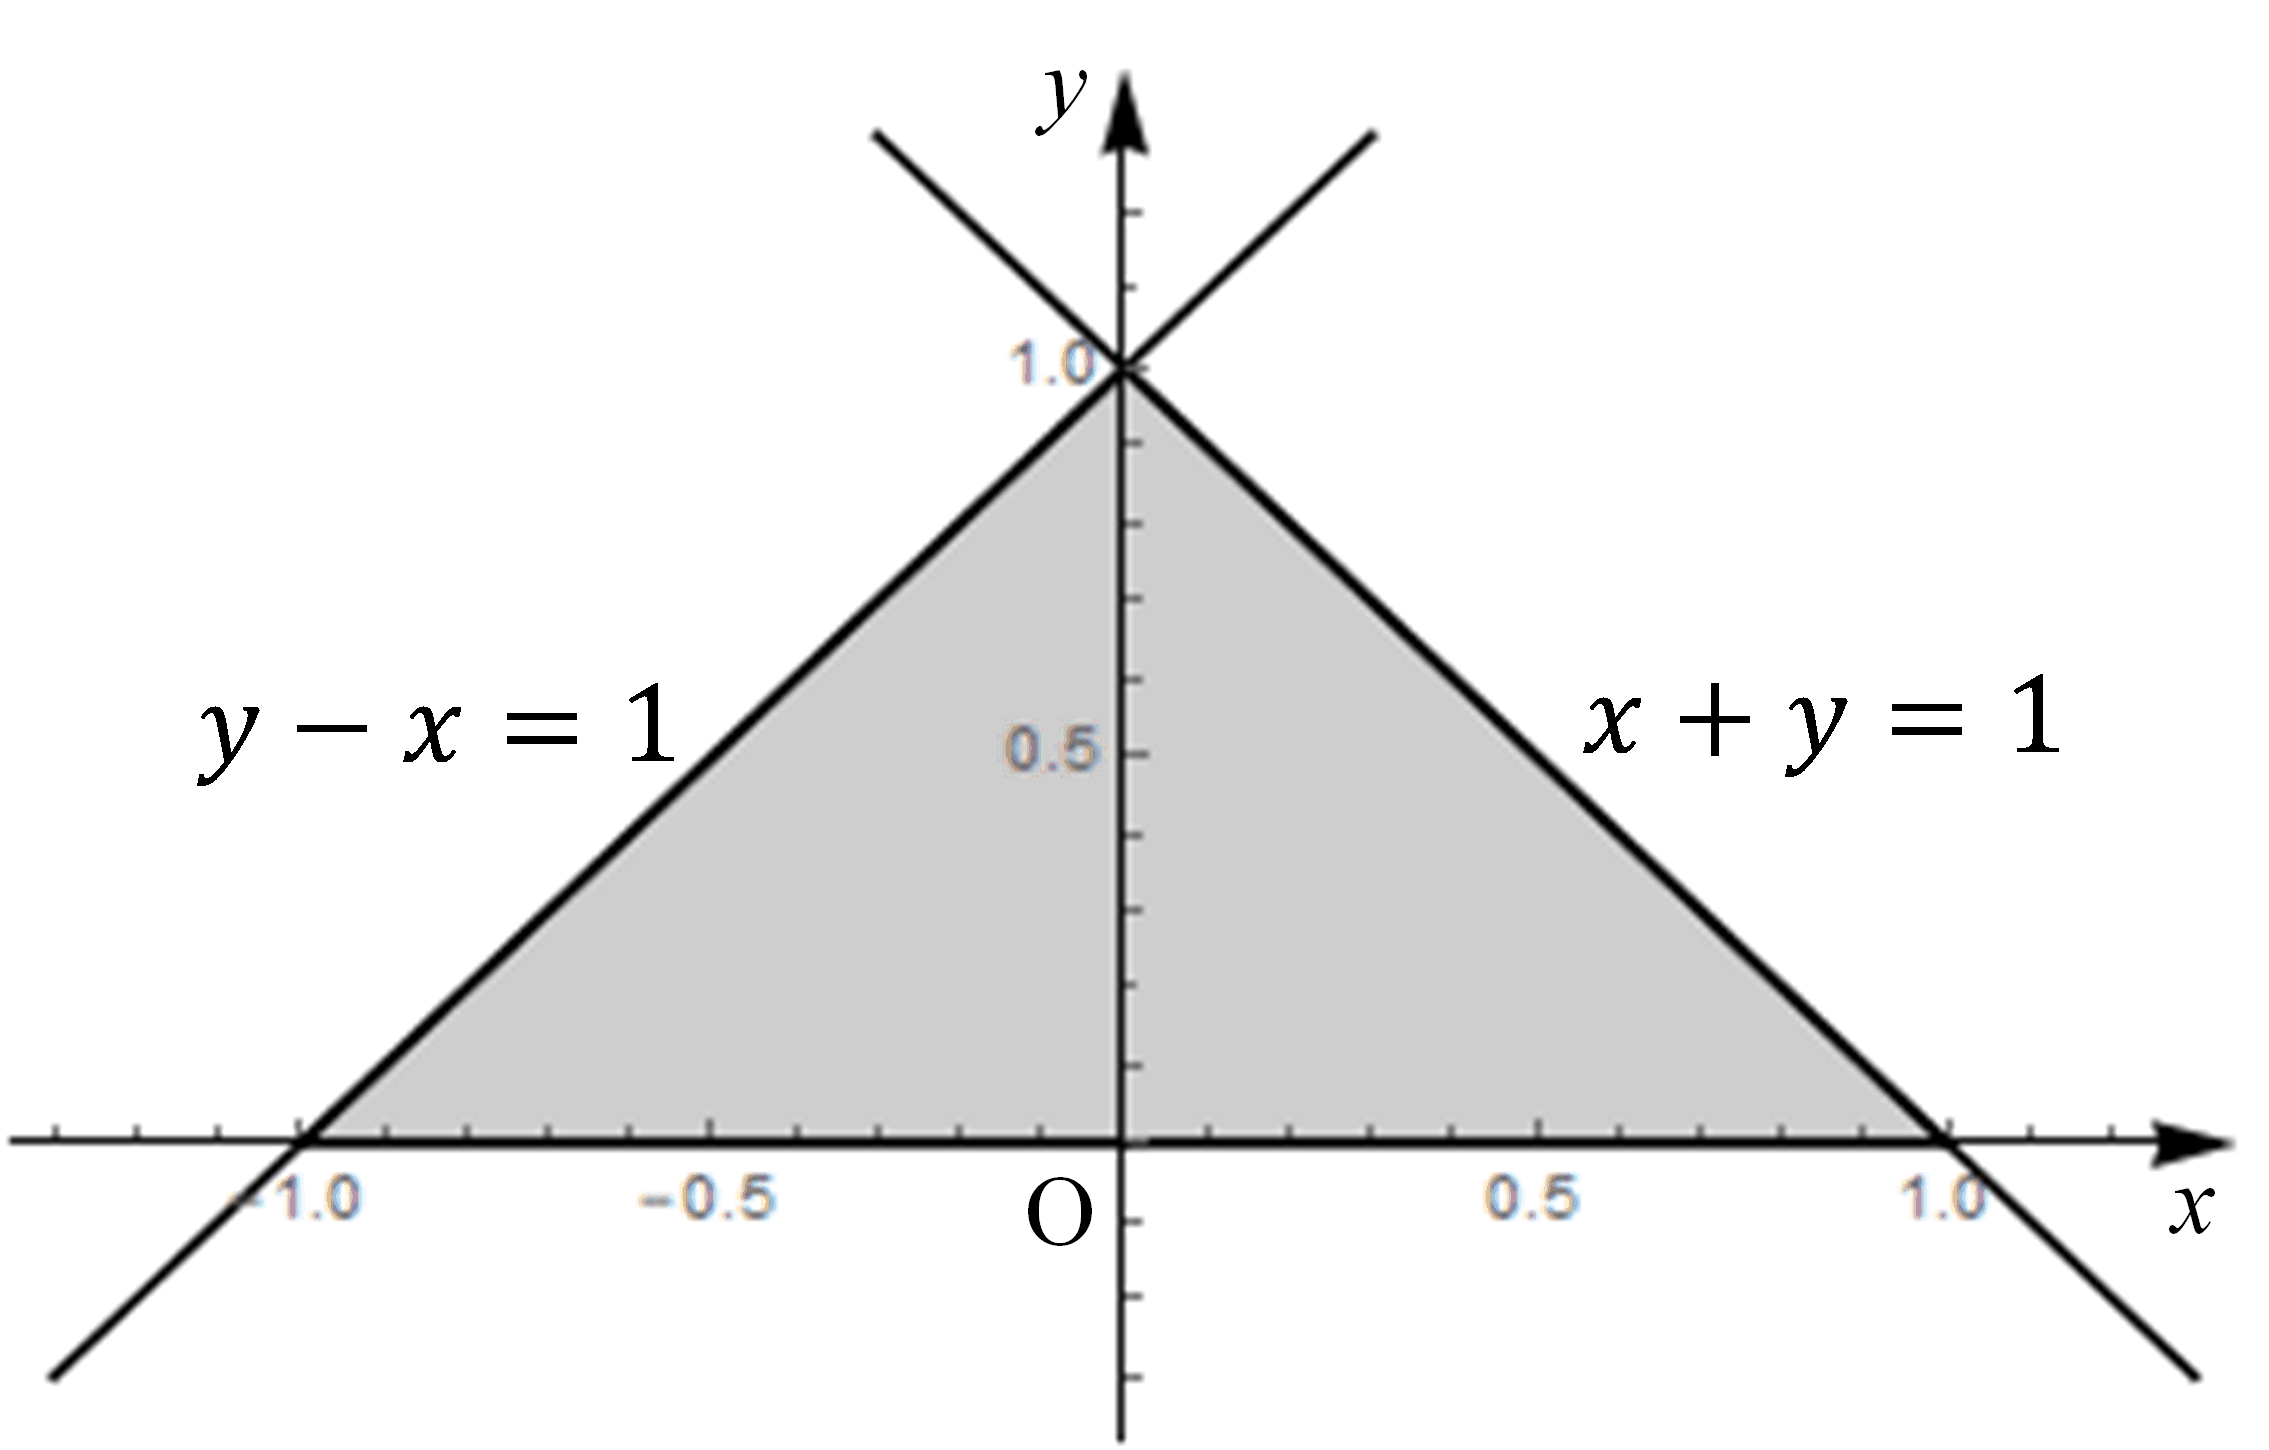
\includegraphics[height=0.2\textheight]{Figures/Fig1-2.png}
\end{center}
\caption{习题12.1 1.(2)题图示}
\label{1-2}
\end{figure}
积分$\aIInt{D}2\mathrm d\sigma$表示以区域$D$为底,高为$2$的棱柱体的体积,故
\[\aIInt{D}2\mathrm d\sigma=2\times(\frac12\times1\times2)=2.\]

\item利用重积分的性质估计下列积分值:\\
(1)$\aIInt{D}(1+y)x\mathrm d\sigma,D=\Set{(x,y)}{x^2+y^2\leqslant1,x\geqslant0,y\geqslant0}$;\\
(2)$\aIInt{D}(x^2+y^2)\mathrm d\sigma,D=\Set{(x,y)}{2x\leqslant x^2+y^2\leqslant4x}$.

解:(1)令$x=r\cos\theta,y=r\sin\theta$,则$D=\Set{(x,y)}{x^2+y^2\leqslant1,x\geqslant0,y\geqslant0}\\
=\Set{(r,\theta)}{0\leqslant r\leqslant1,0\leqslant\theta\leqslant\frac\pi2}$,

$\because$当$0\leqslant r\leqslant1,0\leqslant\theta\leqslant\frac\pi2$时,$0\leqslant\cos\theta\leqslant1,0\leqslant\sin2\theta\leqslant1$,

$\therefore(1+y)x=(1+r\sin\theta)r\cos\theta=r\cos\theta+r^2\sin\theta\cos\theta=r\cos\theta+\frac12r^2\sin2\theta\in[0,\frac32]$,

$\because\aIInt{D}\mathrm d\sigma=\frac\pi4$,

$\therefore0\leqslant\aIInt{D}(1+y)x\mathrm d\sigma\leqslant\frac32\aIInt{D}\mathrm d\sigma=\frac32\cdot\frac\pi4=\frac38\pi$,即$\aIInt{D}(1+y)x\mathrm d\sigma\in[0,\frac38\pi]$.

(2)方法1:$\because 2x\leqslant x^2+y^2\leqslant4x\Leftrightarrow\begin{cases}
x^2+y^2\geqslant2x,\\
x^2+y^2\leqslant4x,
\end{cases}\Leftrightarrow\begin{cases}
(x-1)^2+y^2\geqslant1,\\
(x-2)^2+y^2\leqslant4,
\end{cases}$

$\therefore$区域$D$如图~\ref{2-2}所示,
\begin{figure}[H]
\begin{center}
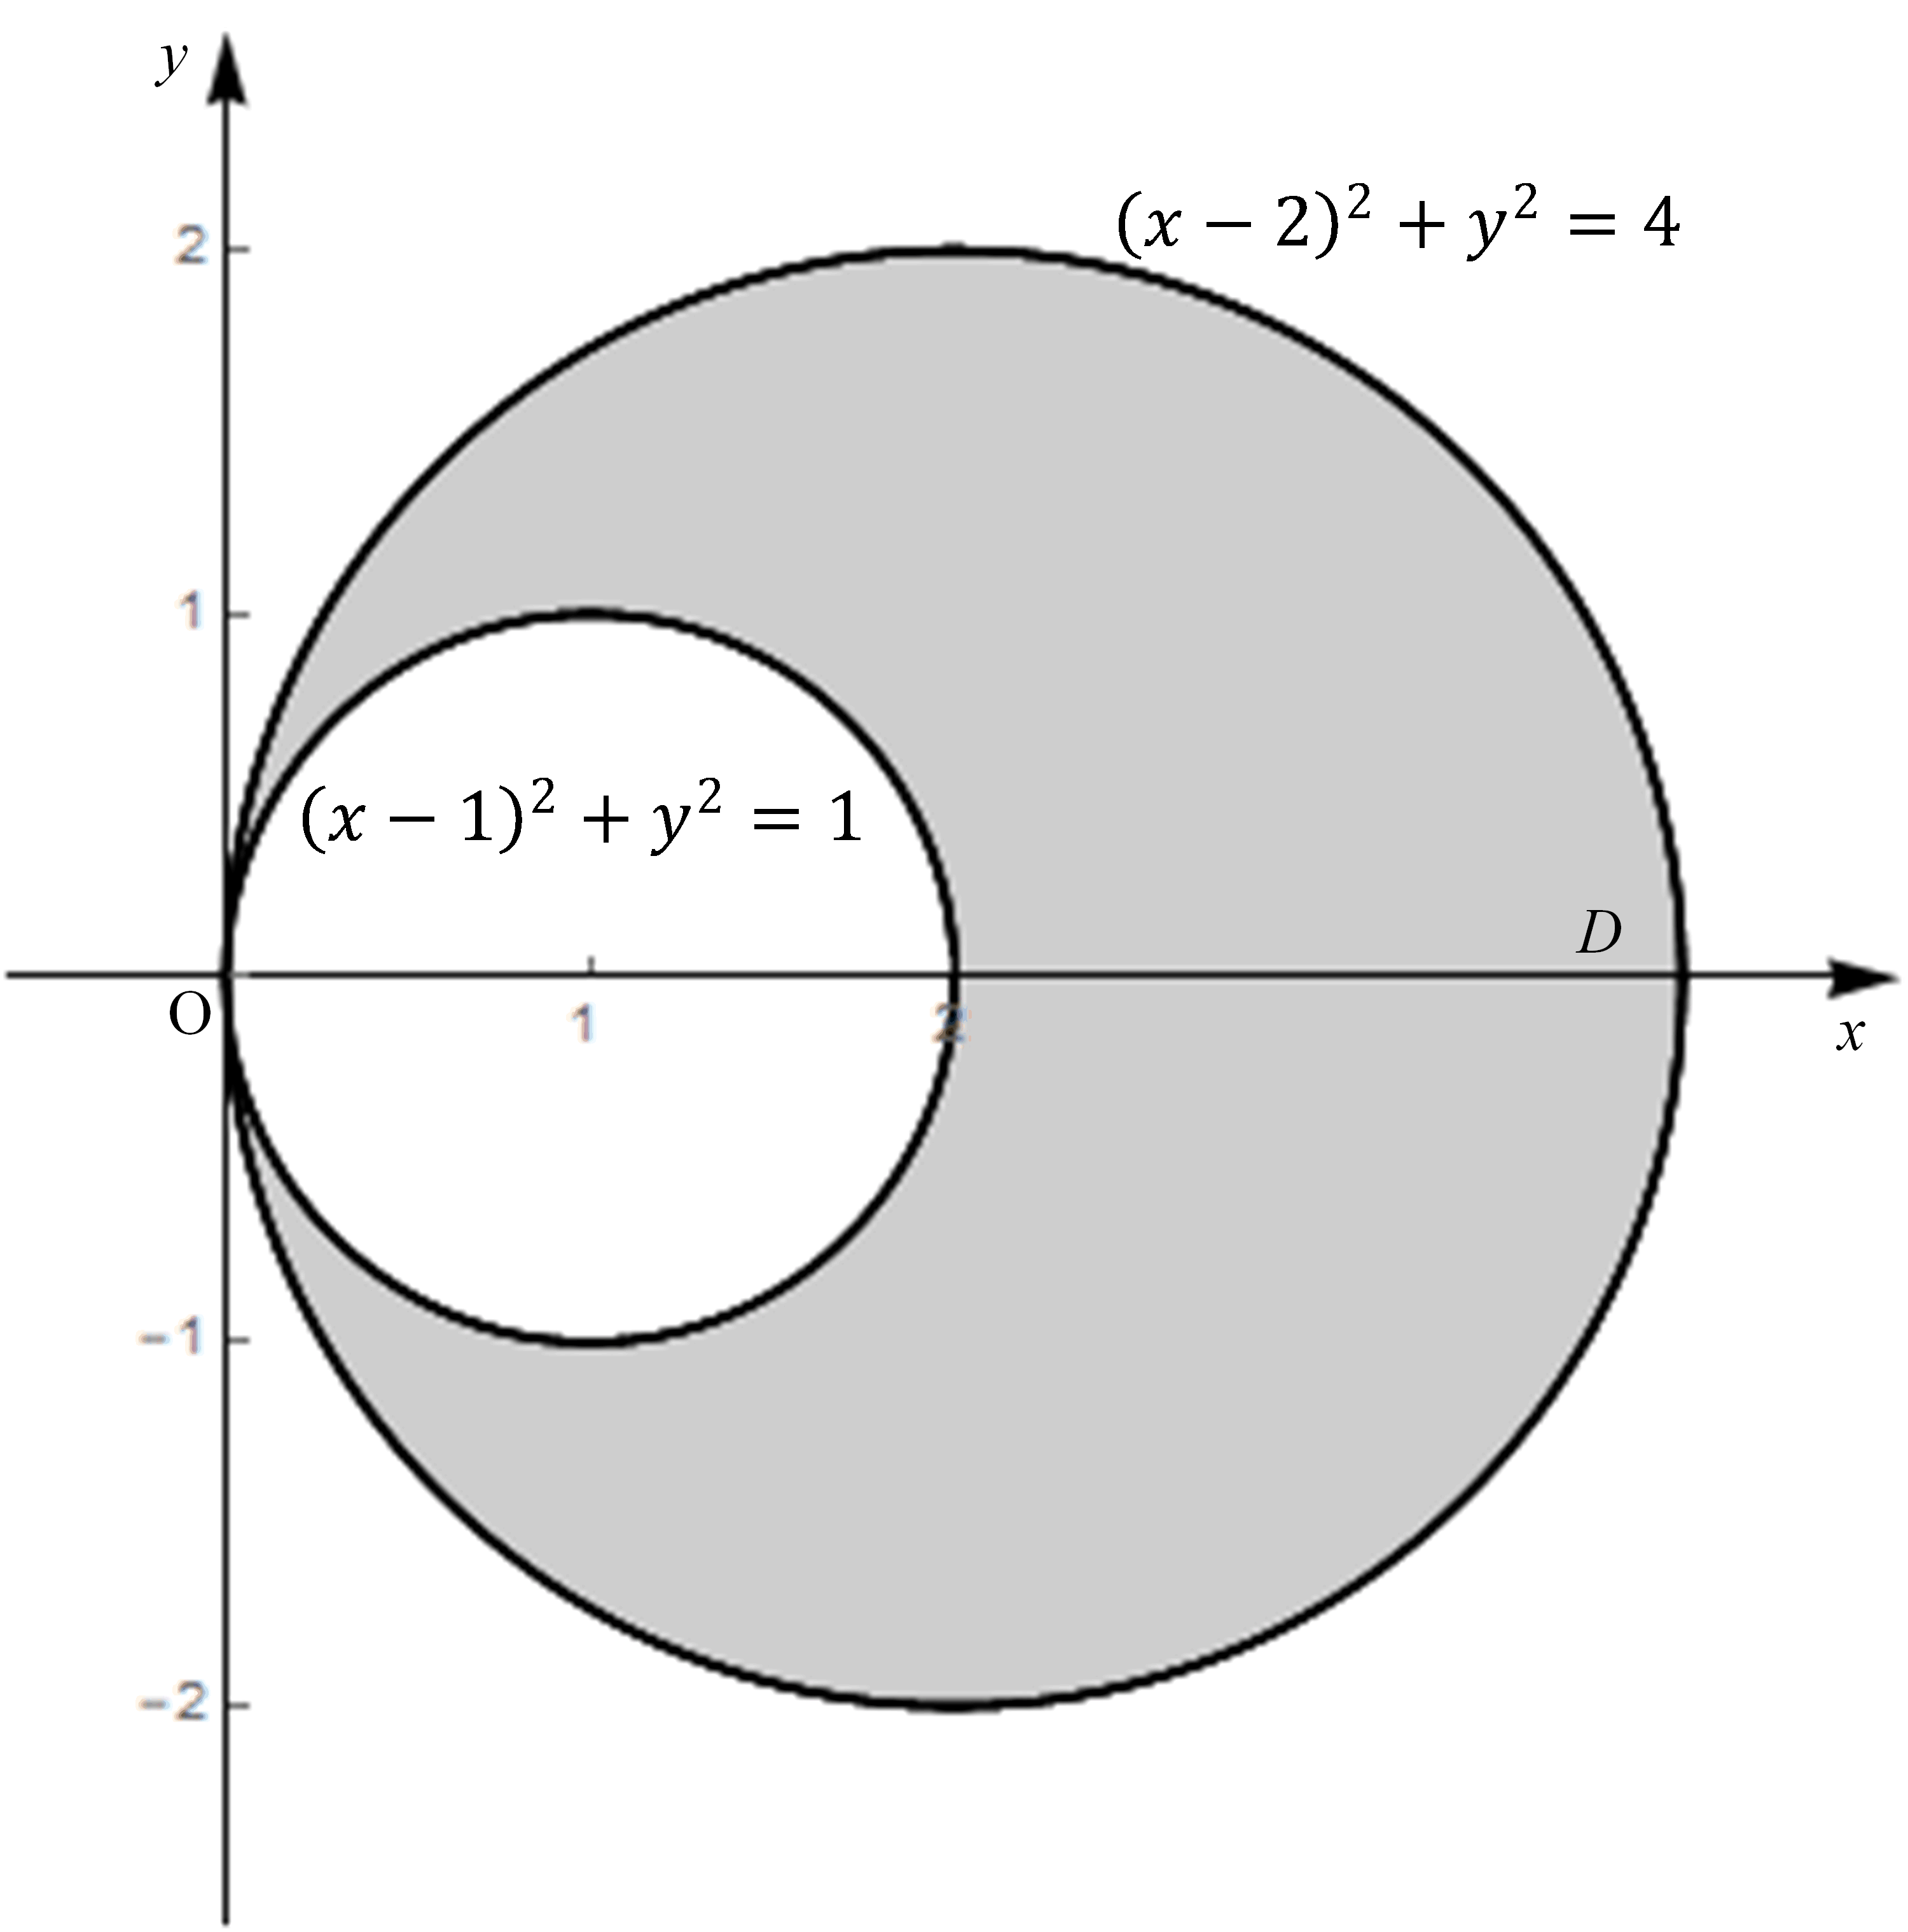
\includegraphics[height=0.3\textheight]{Figures/Fig2-2.png}
\end{center}
\caption{习题12.1 2.(2)题图示}
\label{2-2}
\end{figure}
由图~\ref{2-2}可知$0\leqslant x^2+y^2\leqslant4^2+0^2=16$,

$\because\aIInt{D}\mathrm d\sigma=2^2\pi-1^2\pi=3\pi$,

$\therefore0\leqslant\aIInt{D}(x^2+y^2)\mathrm d\sigma\leqslant16\aIInt{D}\mathrm d\sigma=48\pi$.

方法2:令$x=r\cos\theta,y=r\sin\theta$,则$D=\Set{(x,y)}{2x\leqslant x^2+y^2\leqslant4x}\\
=\Set{(r,\theta)}{2r\cos\theta\leqslant r^2\leqslant4r\cos\theta}=\Set{(r,\theta)}{2\cos\theta\leqslant r\leqslant4\cos\theta,0\leqslant\theta\leqslant2\pi}$,

$\therefore0\leqslant2\cos^2\theta\leqslant r^2\leqslant16\cos^2\theta\leqslant16$,即$0\leqslant x^2+y^2\leqslant4^2+0^2=16$,

$\because\aIInt{D}\mathrm d\sigma=2^2\pi-1^2\pi=3\pi$,

$\therefore0\leqslant\aIInt{D}(x^2+y^2)\mathrm d\sigma\leqslant16\aIInt{D}\mathrm d\sigma=48\pi$.

\item比较下列各组积分值的大小:\\
(1)$\aIInt{D}(x+y)^2\mathrm d\sigma$与$\aIInt{D}(x+y)^3\mathrm d\sigma$,其中$D=\Set{(x,y)}{(x-2)^2+(y-2)^2\leqslant2}$;\\
(2)$\aIInt{D}\ln(x+y)\mathrm d\sigma$与$\aIInt{D}xy\mathrm d\sigma$,其中$D$由直线$x=0,y=0,x+y=\frac12$及$x+y=1$围成.

解:(1)区域$D$的图形如图~\ref{3-1}所示,
\begin{figure}[H]
\begin{center}
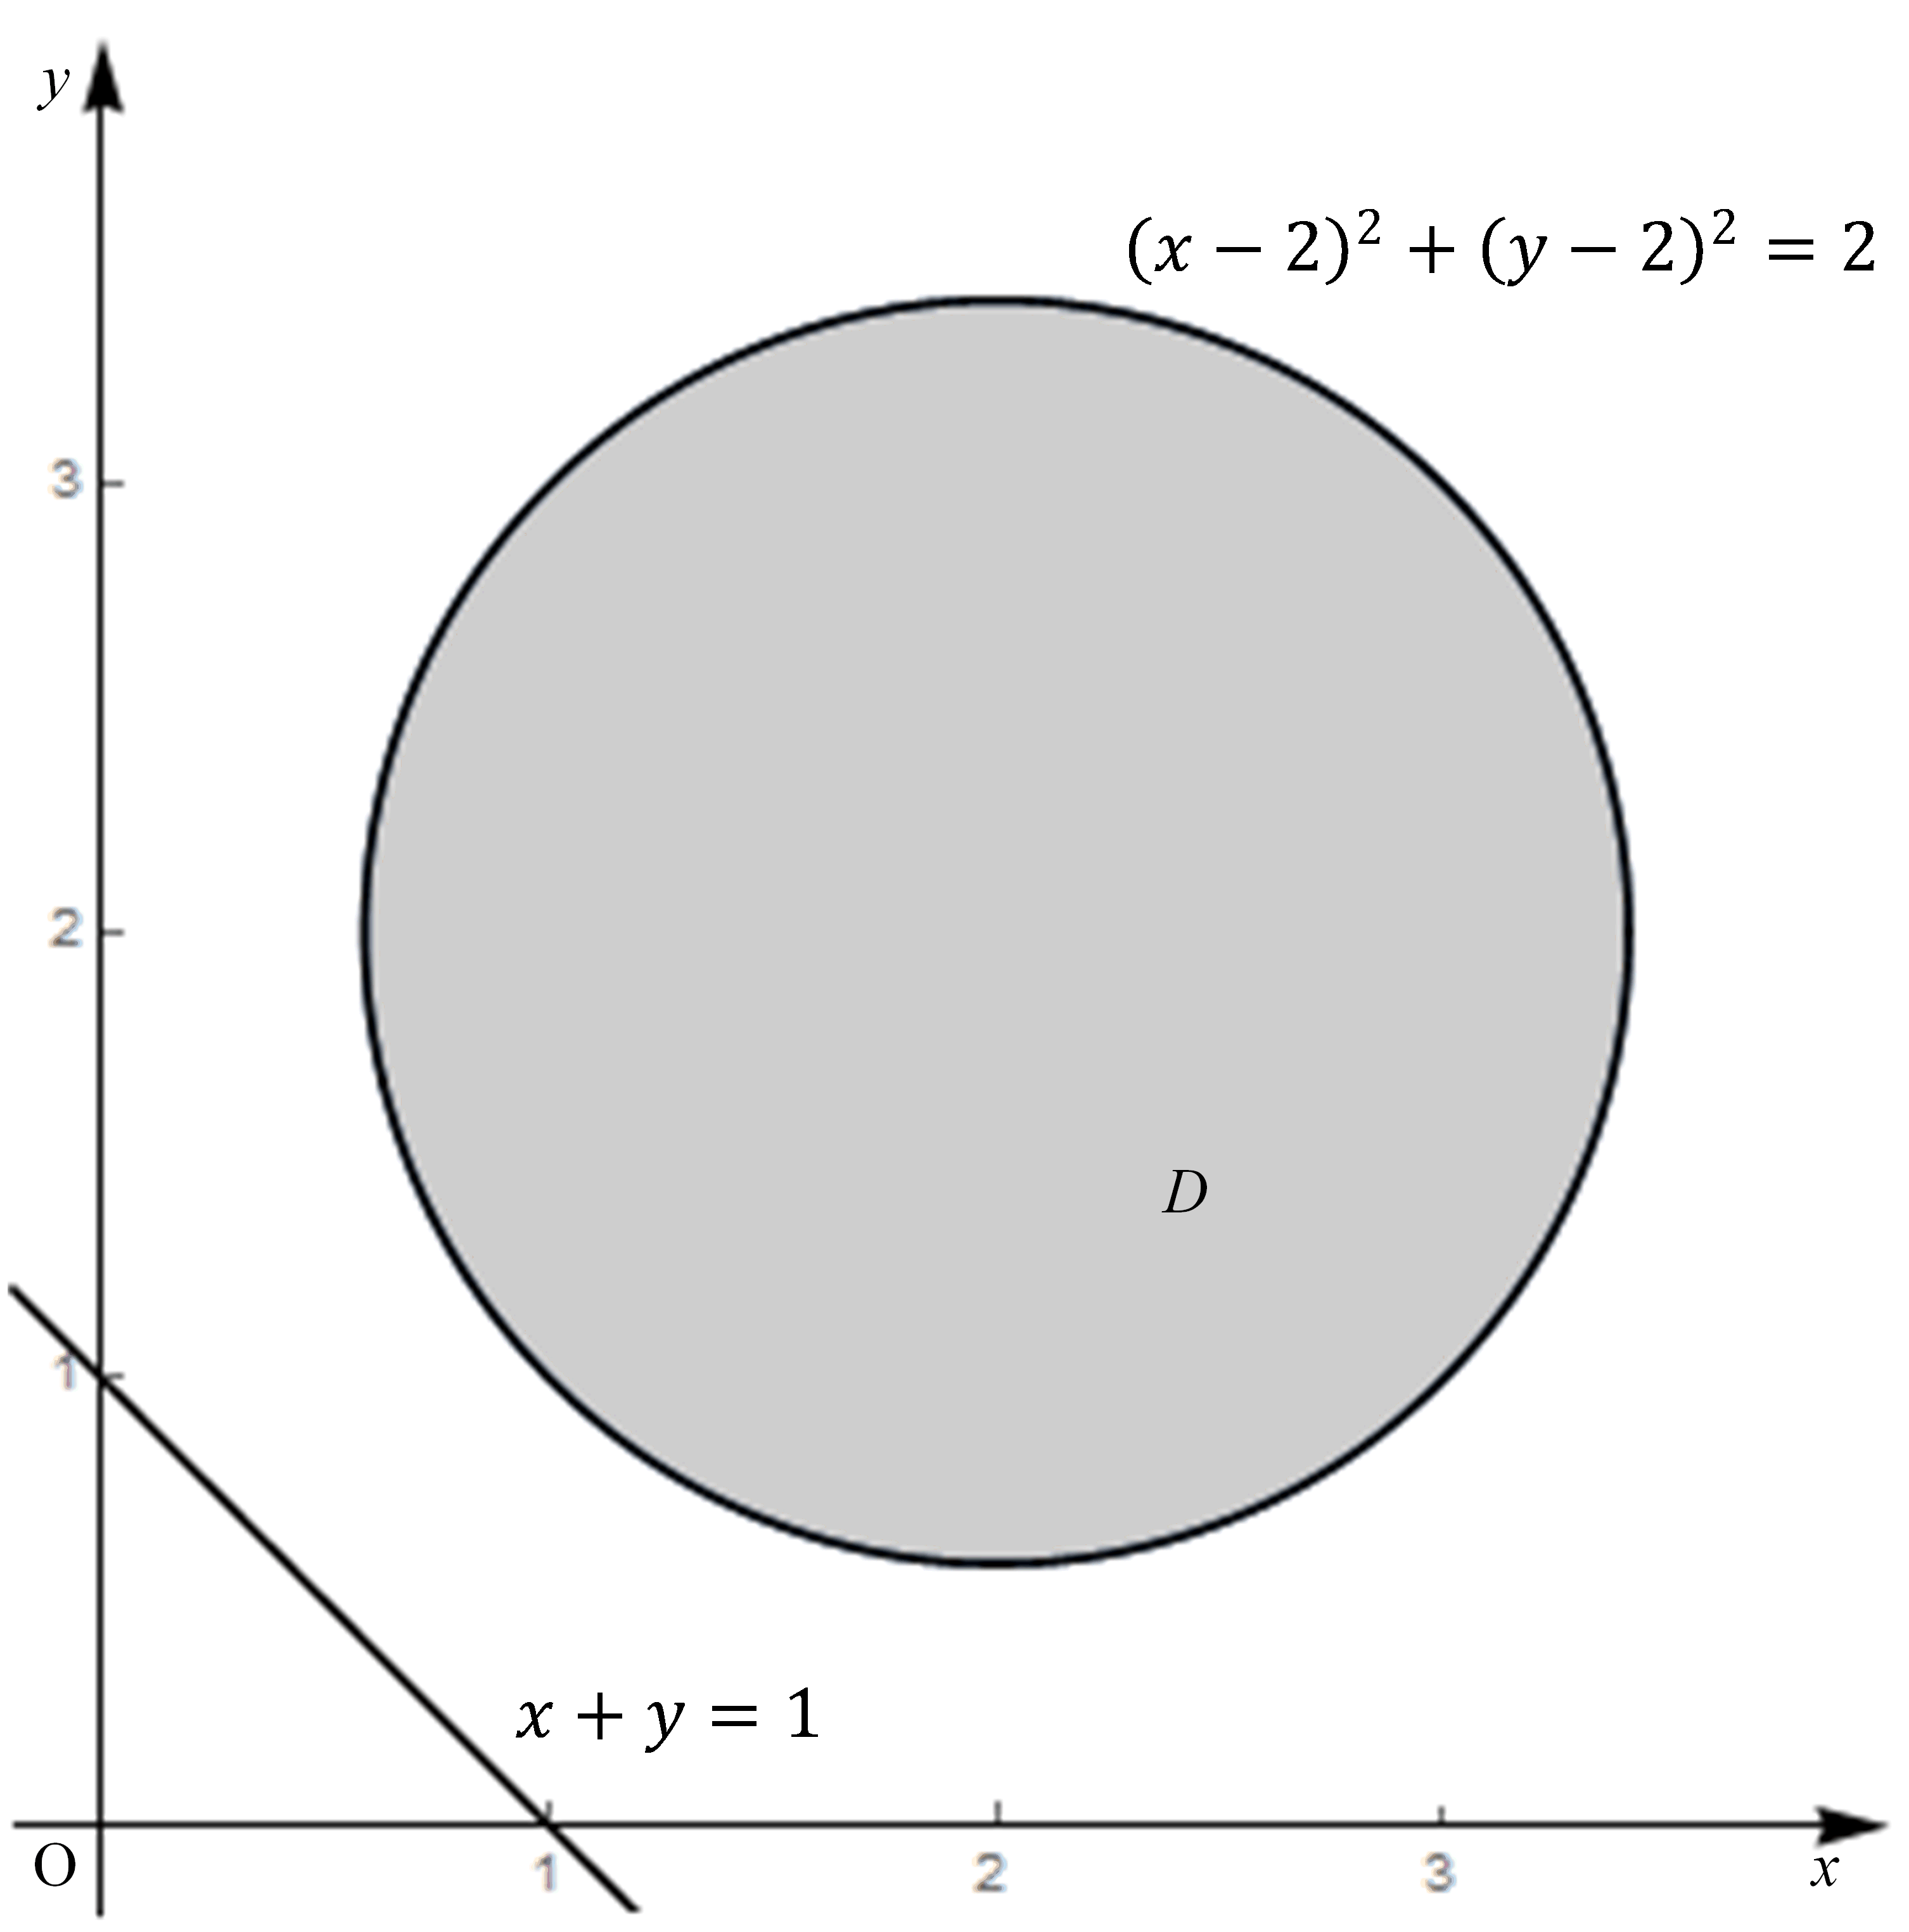
\includegraphics[height=0.3\textheight]{Figures/Fig3-1.png}
\end{center}
\caption{习题12.1 3.(1)题图示}
\label{3-1}
\end{figure}
由图~\ref{3-1}可知在区域$D$上$x+y>1$,则$(x+y)^2<(x+y)^3$,

$\therefore\aIInt{D}(x+y)^2\mathrm d\sigma<\aIInt{D}(x+y)^3\mathrm d\sigma$.

(2)区域$D$的图形如图~\ref{3-2}所示,
\begin{figure}[H]
\begin{center}
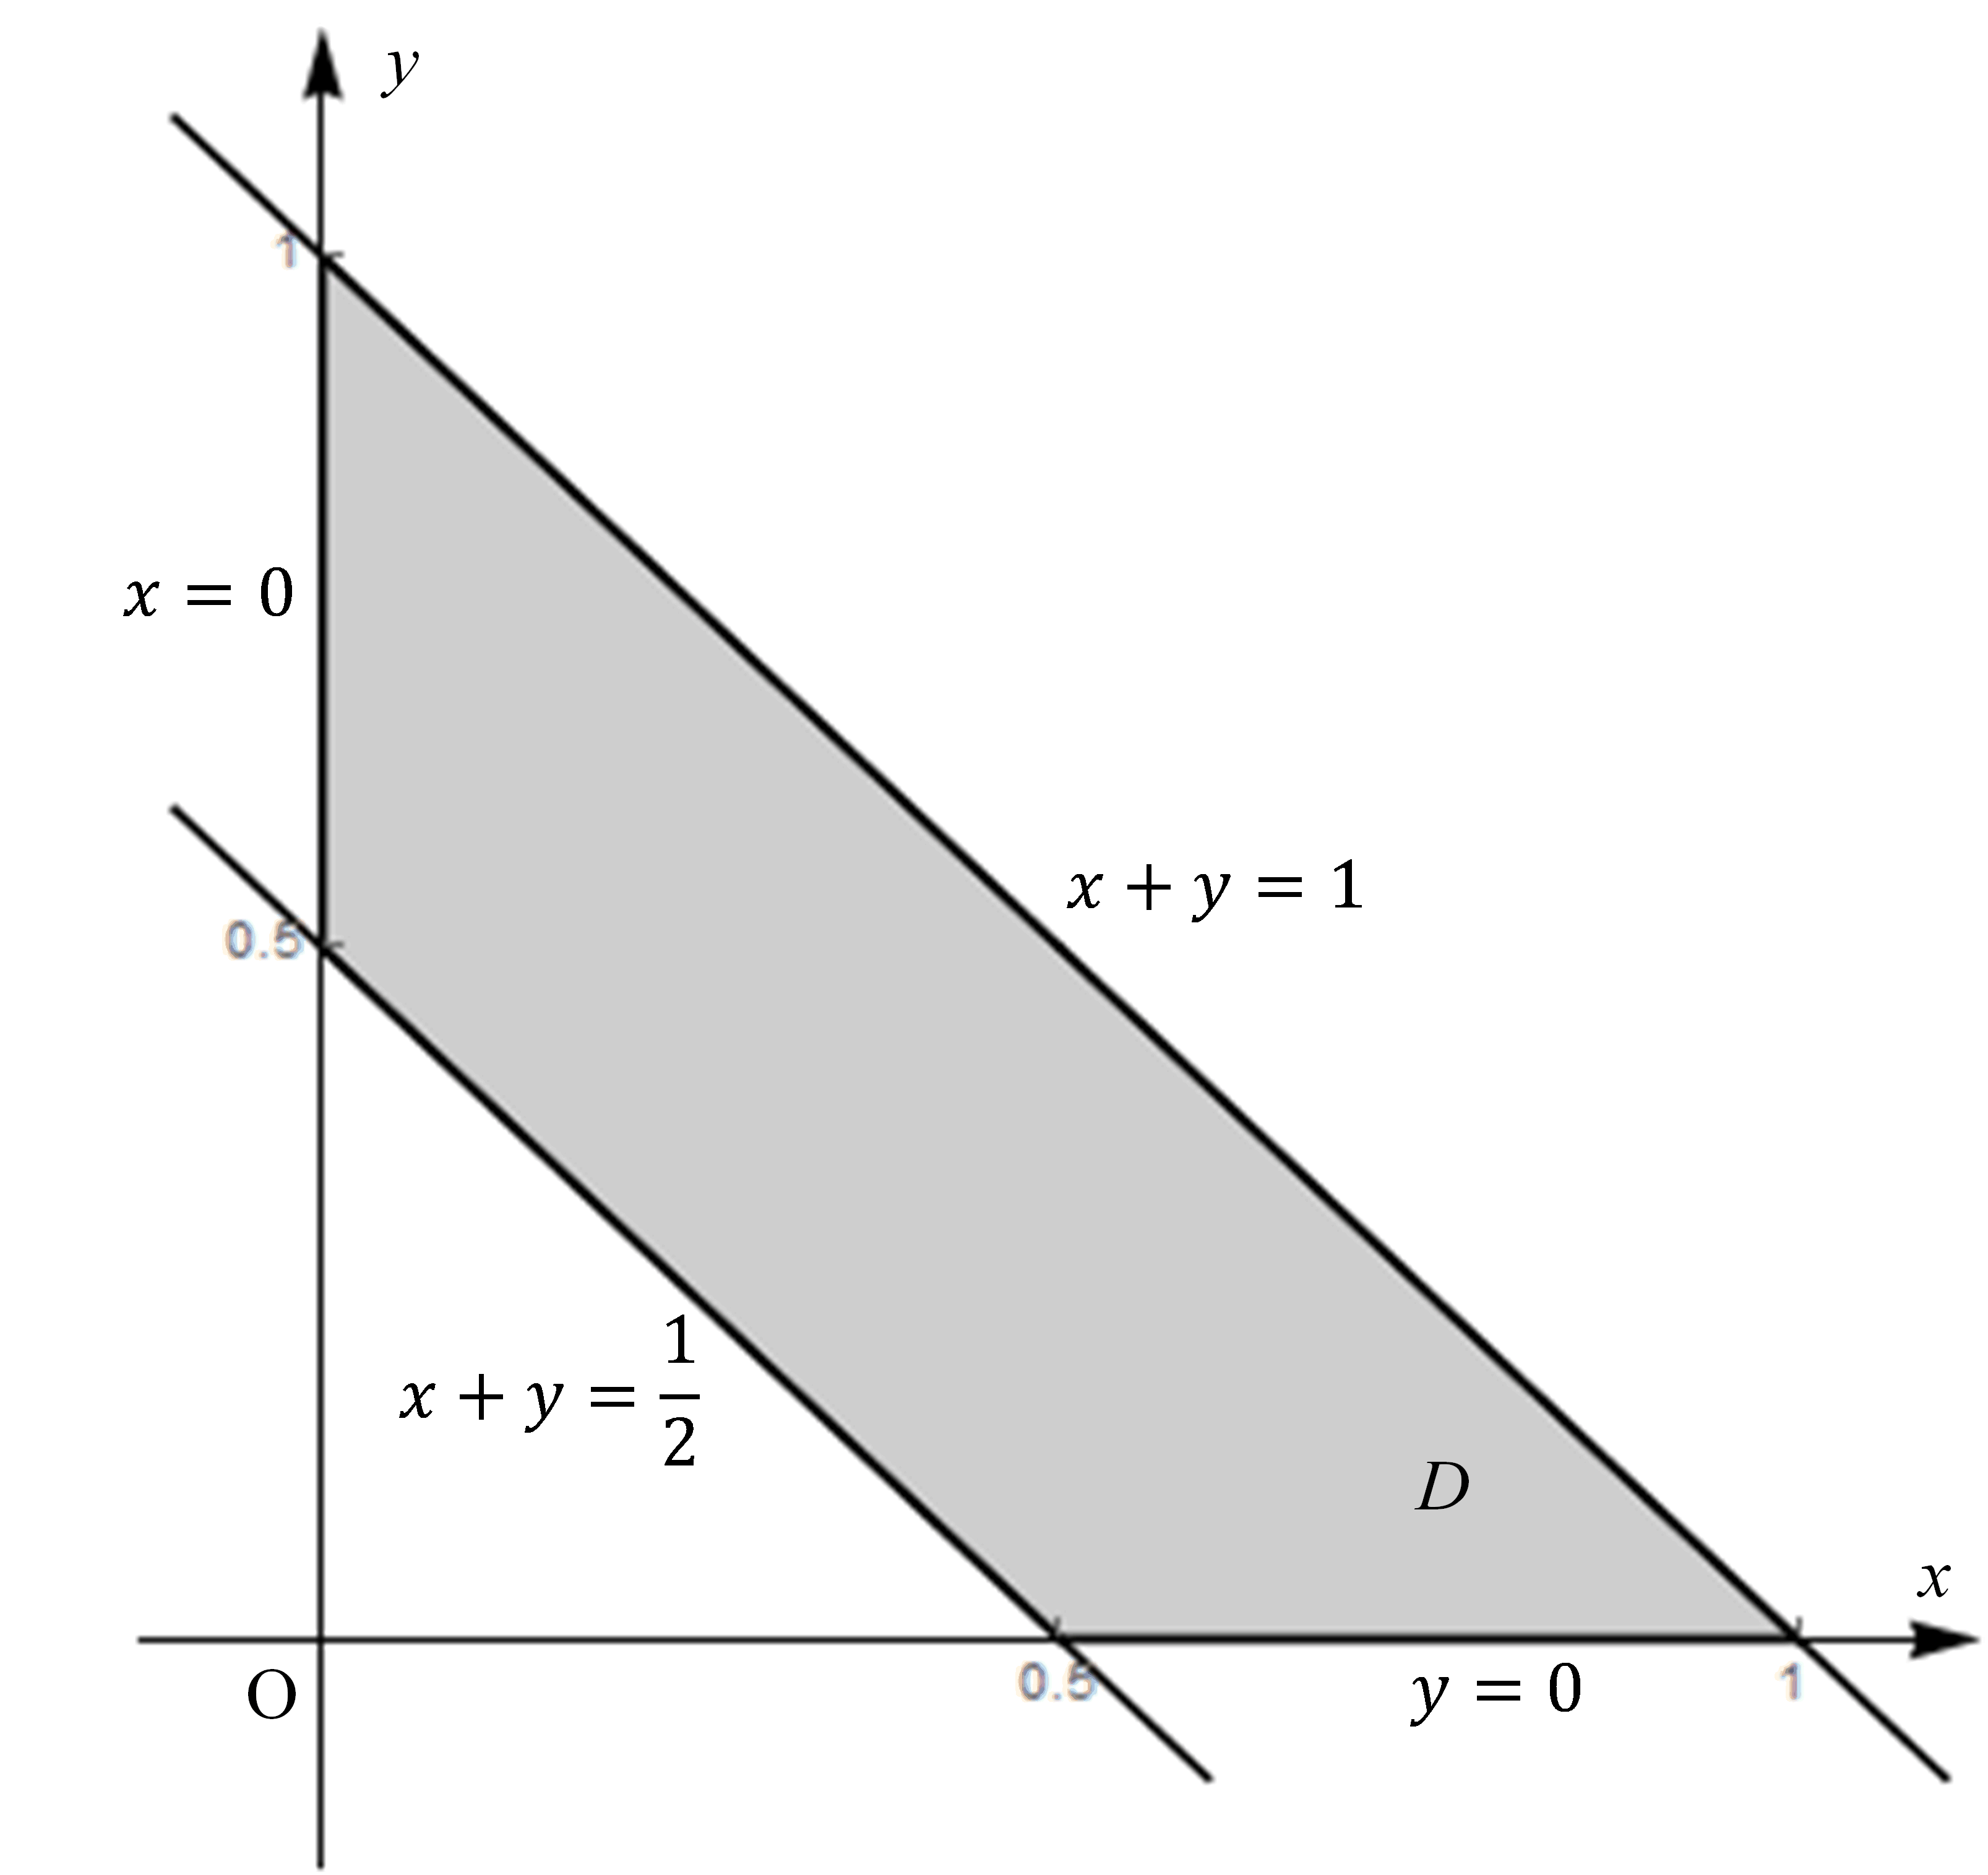
\includegraphics[height=0.3\textheight]{Figures/Fig3-2.png}
\end{center}
\caption{习题12.1 3.(2)题图示}
\label{3-2}
\end{figure}
由图~\ref{3-1}可知在区域$D$上$0<x+y\leqslant1$,则$\ln(x+y)\leqslant0\leqslant xy$,

$\therefore\aIInt{D}\ln(x+y)\mathrm d\sigma<0<\aIInt{D}xy\mathrm d\sigma$.

\item设$D\subset\mathbb R^2$是一有界闭域,$f(x,y)\in C(D)$且非负,试证:若$\aIInt{D}f(x,y)\mathrm d\sigma=0$,则\\
$f(x,y)\equiv0,\forall(x,y)\in D$.

证明:假设$f(x,y)$不恒为$0$,

$\because f(x,y)\in C(D)$且非负,

$\therefore\exists P(x_0,y_0)\in D$满足$f(x_0,y_0)>0$,且存在$P(x_0,y_0)$的一个邻域$N(P,\delta)$使得\\
$f(x,y)>\frac12f(x_0,y_0)>0$,

$\therefore\aIInt{D}f(x,y)\mathrm d\sigma=\aIInt{N(P,\delta)}f(x,y)\mathrm d\sigma+\aIInt{D\setminus N(P,\delta)}f(x,y)\mathrm d\sigma\geqslant\aIInt{N(P,\delta)}f(x,y)\mathrm d\sigma+0>0$,这与$\aIInt{D}f(x,y)\mathrm d\sigma=0$矛盾,

$\therefore$假设不成立,

$\therefore f(x,y)\equiv0,\forall(x,y)\in D$.
\item证明:若$f(x,y)\in C(D),g(x,y)\in R(D)$且不变号,则$\exists(\xi,\eta)\in D$使得
\[
\aIInt{D}f(x,y)g(x,y)\mathrm d\sigma=f(\xi,\eta)\aIInt{D}g(x,y)\mathrm d\sigma.
\]

证明:$\because f(x,y)\in C(D)$,

$\therefore\exists P,Q\in D,s.t.\ f(P)=m,f(Q)=M,\text{且}m\leqslant f(x,y)\leqslant M,\forall (x,y)\in D$,

$\because g(x,y)\in R(D)$且不变号,不妨设$g(x,y)\geqslant 0$,

$\therefore mg(x,y)\leqslant f(x,y)g(x,y)\leqslant Mg(x,y)$,

$\therefore m\aIInt{D}g(x,y)\mathrm d\sigma\leqslant\aIInt{D}f(x,y)g(x,y)\mathrm d\sigma\leqslant M\aIInt{D}g(x,y)\mathrm d\sigma$,

$\therefore$

i)当$\aIInt{D}g(x,y)\mathrm d\sigma=0$时$\aIInt{D}f(x,y)g(x,y)\mathrm d\sigma=0$,故$\aIInt{D}f(x,y)g(x,y)\mathrm d\sigma=f(\xi,\eta)\aIInt{D}g(x,y)\mathrm d\sigma$成立;

ii)当$\aIInt{D}g(x,y)\mathrm d\sigma\neq0$时$m\leqslant\frac{\aIInt{D}f(x,y)g(x,y)\mathrm d\sigma}{\aIInt{D}g(x,y)\mathrm d\sigma}\leqslant M$,由连续函数的介值定理知$\exists(\xi,\eta)\in D$满足
\[f(\xi,\eta)=\frac{\aIInt{D}f(x,y)g(x,y)\mathrm d\sigma}{\aIInt{D}g(x,y)\mathrm d\sigma},\]
即
\[\aIInt{D}f(x,y)g(x,y)\mathrm d\sigma=f(\xi,\eta)\aIInt{D}g(x,y)\mathrm d\sigma.\]
\item利用性质7的结论计算下列积分(其中区域$D$为圆盘$x^2+y^2\leqslant R^2$):\\
\begin{tabular}{ll}
(1)$\aIInt{D}y\sqrt{R^2-x^2}\mathrm d\sigma$;&(2)$\aIInt{D}y^3x^2\mathrm d\sigma$;\\
(3)$\aIInt{D}x^5\sqrt{R^2-y^2}\mathrm d\sigma$;&(4)$\aIInt{D}x^my^n\mathrm d\sigma$.
\end{tabular}

解:(1)因为区域$D$关于$x$轴对称,被积函数$f(x,y)=y\sqrt{R^2-x^2}=-f(x,-y)$关于$y$是奇函数,故$\aIInt{D}y\sqrt{R^2-x^2}\mathrm d\sigma=0$.

(2)因为区域$D$关于$x$轴对称,被积函数$f(x,y)=y^3x^2=-f(x,-y)$关于$y$是奇函数,故$\aIInt{D}y^3x^2\mathrm d\sigma=0$.

(3)因为区域$D$关于$y$轴对称,被积函数$f(x,y)=x^5\sqrt{R^2-y^2}=-f(-x,y)$关于$x$是奇函数,故$\aIInt{D}x^5\sqrt{R^2-y^2}\mathrm d\sigma=0$.

(4)区域$D$关于$x$轴和$y$轴均对称,

i)当$m$与$n$都是偶数时,$f(x,y)=x^my^n=f(-x,y)=f(x,-y)$关于$x$和$y$均是偶函数,故\\
$\aIInt{D}x^my^n\mathrm d\sigma=4\aIInt{D_1}x^my^n\mathrm d\sigma$,其中$D_1=\Set{(x,y)}{x^2+y^2\leqslant R^2,x\geqslant0,y\geqslant0}$;

ii)当$m$与$n$都是奇数时,$f(x,y)=x^my^n=-f(-x,y)$关于$x$是奇函数,$\aIInt{D}x^my^n\mathrm d\sigma=0$;

iii)当$m$是奇数$n$是偶数时,$f(x,y)=x^my^n=-f(-x,y)$关于$x$是奇函数,$\aIInt{D}x^my^n\mathrm d\sigma=0$;

iv)当$m$是偶数$n$是奇数时,$f(x,y)=x^my^n=-f(x,-y)$关于$y$是奇函数,$\aIInt{D}x^my^n\mathrm d\sigma=0$.

综上所述,当$m,n$均为偶数时,$\aIInt{D}x^my^n\mathrm d\sigma=4\aIInt{D_1}x^my^n\mathrm d\sigma$,其中$D_1$为区域$D$落在第一象限的部分;当$m,n$中至少有一个奇数时,$\aIInt{D}x^my^n\mathrm d\sigma=0$.
\end{enumerate}
\subsection{习题12.2解答}
\begin{enumerate}
\item计算下列二重积分:\\
(1)$\aIInt{D}\cos(x+y)\mathrm d\sigma,D$是由$x=0,y=\pi$和$y=x$围成的区域;\\
(2)$\aIInt{D}xy\ln(1+x^2+y^2)\mathrm d\sigma,D$是由$y=x^3,y=1$和$x=-1$围成的区域;\\
(3)$\aIInt{D}\sin(x+y)\mathrm d\sigma$,其中$D$由直线$x=0,y=x,y=\pi$围成;\\
(4)$\aIInt{D}|x^2-y|\mathrm d\sigma,D=\Set{(x,y)}{0\leqslant x,y\leqslant1}$;\\
(5)$\aIInt{D}\frac{x\sin y}y\mathrm d\sigma$,其中$D$由$y=x,y=x^2$围成.

解:(1)方法1:$\aIInt{D}\cos(x+y)\mathrm d\sigma=\Int{0}{\pi}{}{x}\Int{x}{\pi}{\cos(x+y)}{y}=\Int{0}{\pi}{\sin(x+y)\big|_x^\pi}{x}\\
=\Int{0}{\pi}{[\sin(x+\pi)-\sin2x]}{x}=\Int{0}{\pi}{(-\sin x-\sin2x)}{x}=\cos x\big|_0^\pi+\frac12\cos2x\big|_0^\pi\\
=-1-1+\frac12(1-1)=-2$.

方法2:$\aIInt{D}\cos(x+y)\mathrm d\sigma=\Int{0}{\pi}{}{y}\Int{0}{y}{\cos(x+y)}{x}=\Int{0}{\pi}{\sin(x+y)\big|_0^y}{y}\\
=\Int{0}{\pi}{(\sin2y-\sin x)}{y}=-\frac12\cos2y\big|_0^\pi+\cos x\big|_0^\pi=-\frac12(1-1)+(-1-1)=-2$.

(2)区域$D$如图~\ref{12-2-1-2}所示,
\begin{figure}[H]
\begin{center}
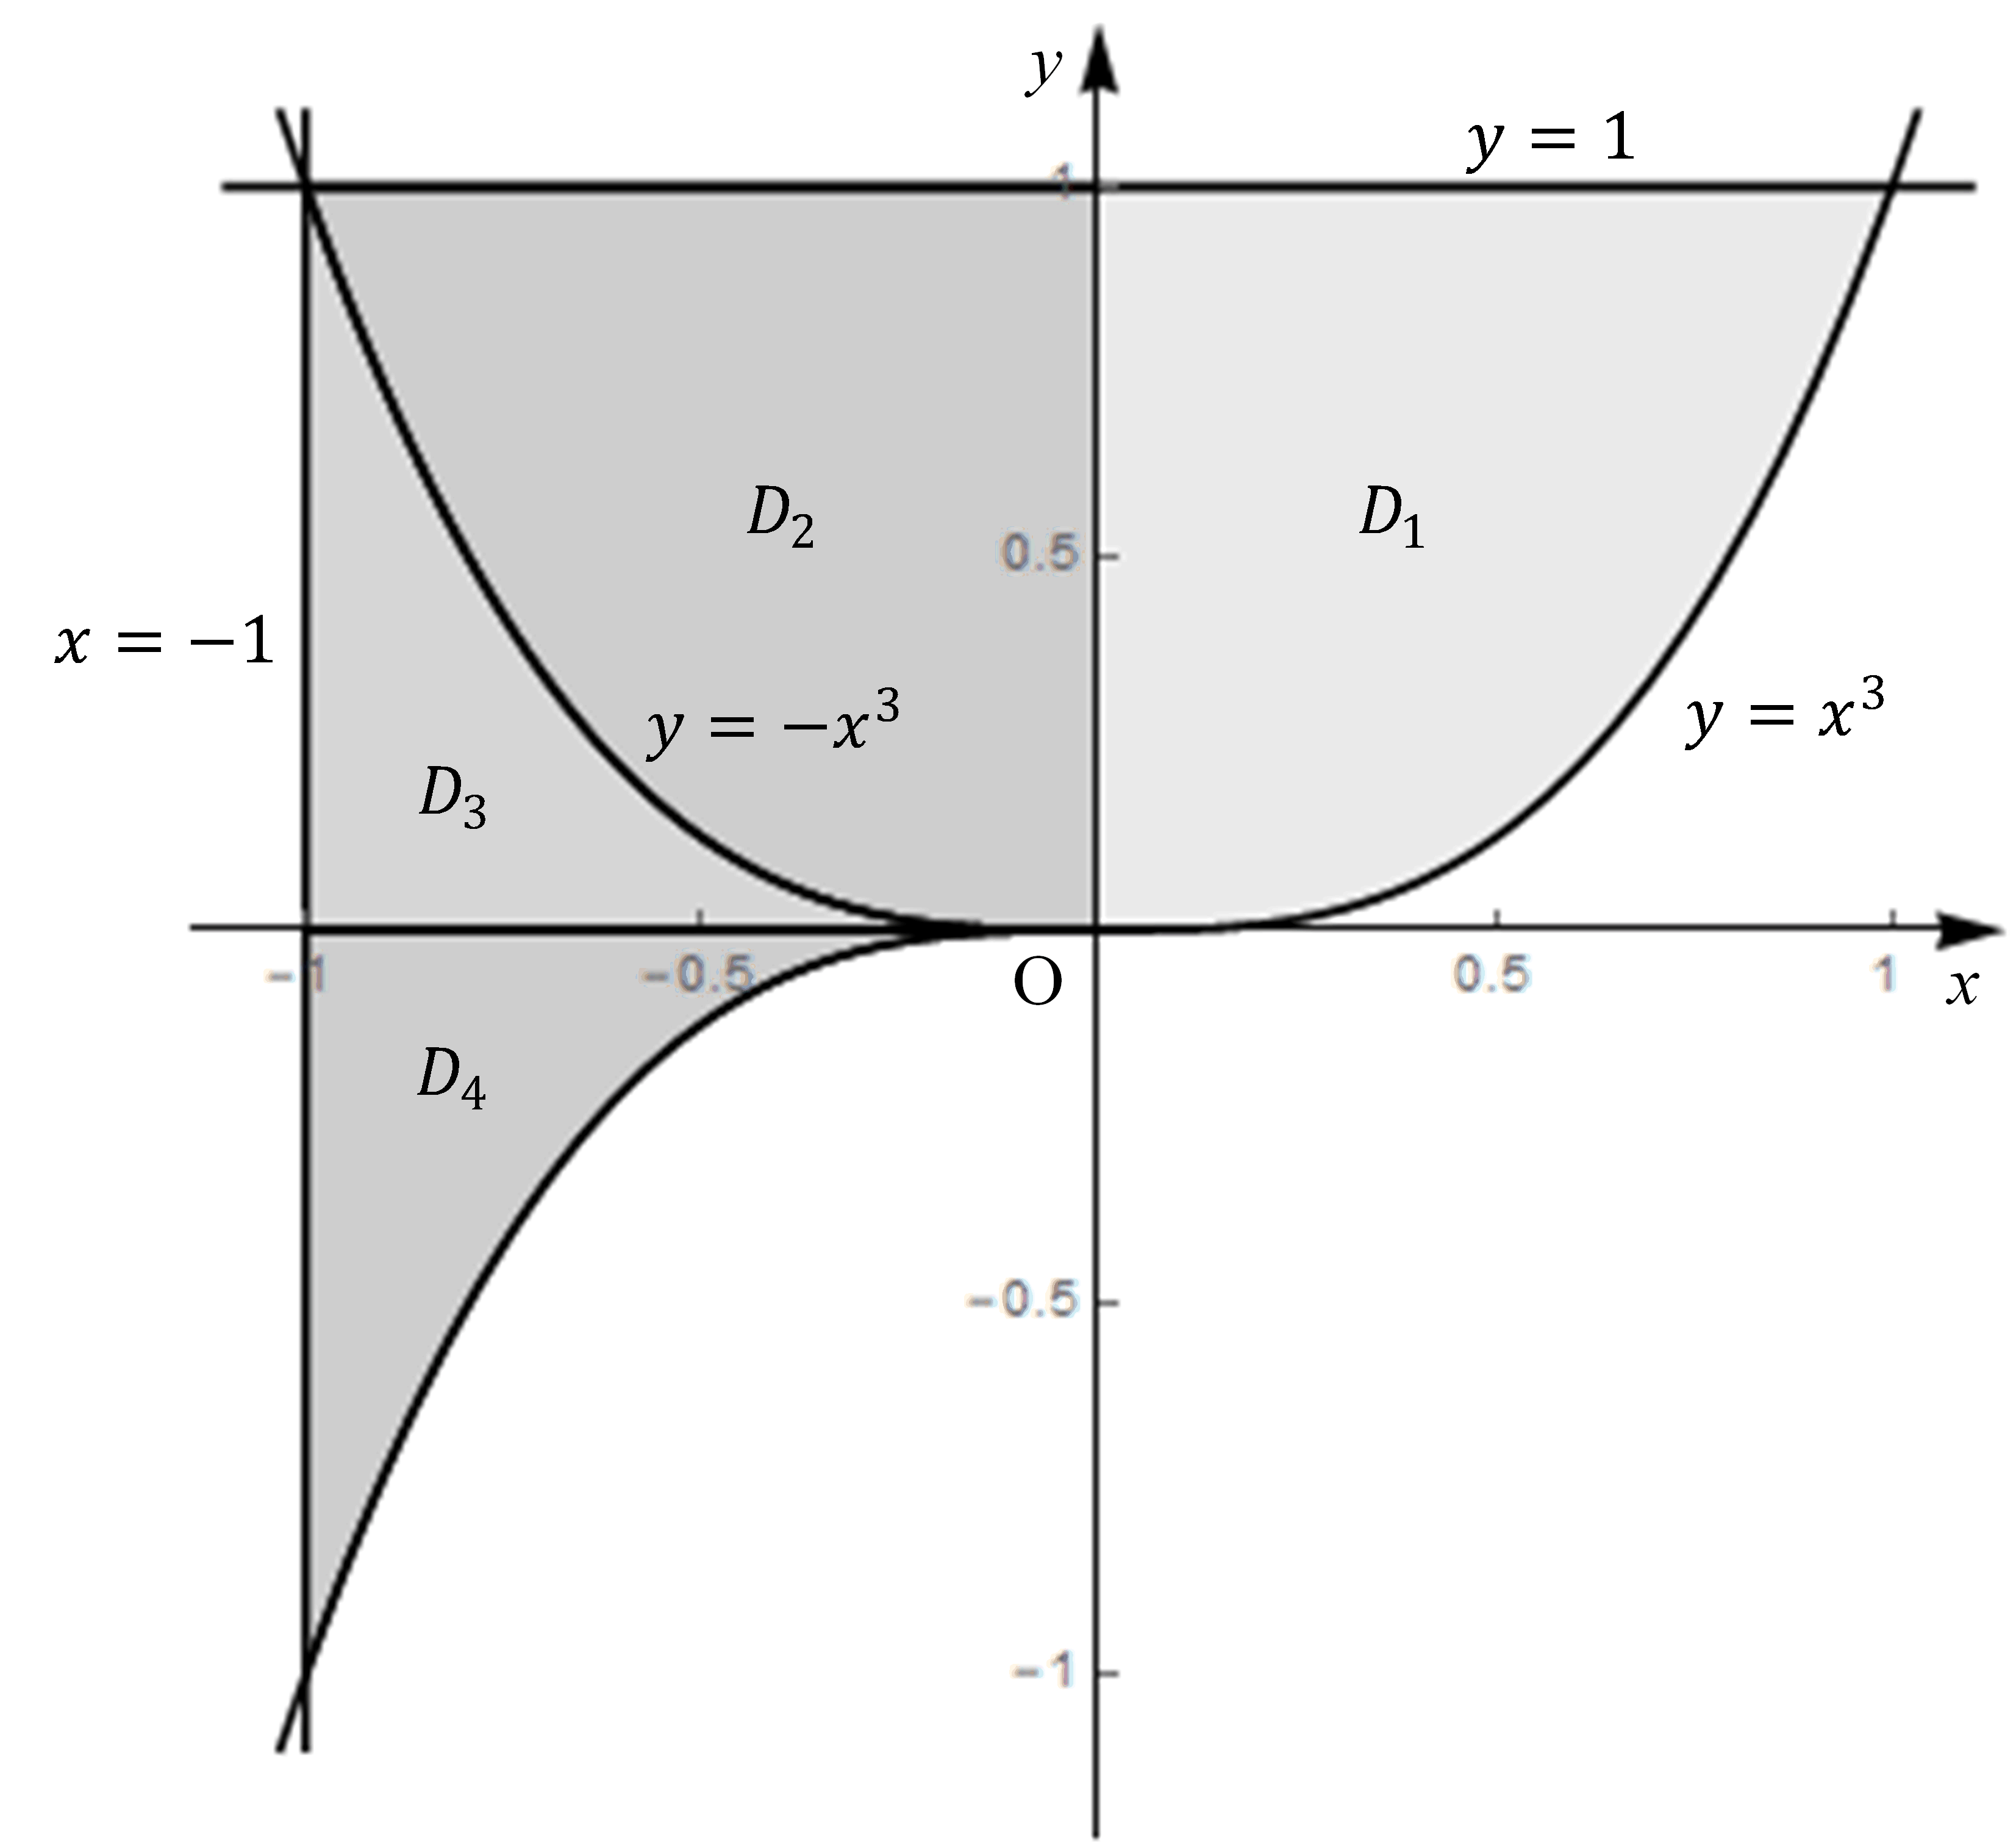
\includegraphics[height=0.3\textheight]{Figures/Fig12-2-1-2.png}
\end{center}
\caption{习题12.2 1.(2)题图示}
\label{12-2-1-2}
\end{figure}
可将区域$D$划分为图中的四个区域,其中$D_1$与$D_2$关于$y$轴对称,$D_3$与$D_4$关于$x$轴对称,被积函数$f(x,y)=xy\ln(1+x^2+y^2)$关于$x$和$y$均为奇函数,

$\therefore\IInt{D_1}xy\ln(1+x^2+y^2)\mathrm d\sigma+\IInt{D_2}xy\ln(1+x^2+y^2)\mathrm d\sigma=0,\\
\aIInt{D_3}xy\ln(1+x^2+y^2)\mathrm d\sigma+\aIInt{D_4}xy\ln(1+x^2+y^2)\mathrm d\sigma=0$,

$\therefore\aIInt{D}xy\ln(1+x^2+y^2)\mathrm d\sigma\\
=\aIInt{D_1}xy\ln(1+x^2+y^2)\mathrm d\sigma+\aIInt{D_2}xy\ln(1+x^2+y^2)\mathrm d\sigma+\aIInt{D_3}xy\ln(1+x^2+y^2)\mathrm d\sigma\\
+\aIInt{D_4}xy\ln(1+x^2+y^2)\mathrm d\sigma=0$.

(3)方法1:$\IInt{D}{\sin(x+y)}{\sigma}=\Int0\pi{}y\Int0y{\sin(x+y)}x=\Int0\pi{-\cos(x+y)\big|_0^y}y\\
=\Int0\pi{(-\cos y+\cos2y)}y=(-\sin y+\frac12\sin2y)\big|_0^\pi=0$.

方法2:$\IInt{D}{\sin(x+y)}{\sigma}=\Int0\pi{}x\Int x\pi{\sin(x+y)}x=\Int0\pi{-\cos(x+y)\big|_x^\pi}x\\
=\Int0\pi{[-\cos(\pi+x)+\cos2x]}x=\Int0\pi{(\cos x+\cos2x)}x=(\sin x+\frac12\sin2x)\big|_0^\pi=0$.

(4)将积分域$D$划分为以下两个区域$D_1=\Set{(x,y)}{0\leqslant x\leqslant1,0\leqslant y\leqslant x^2}$\\
和$D_2=\Set{(x,y)}{0\leqslant x\leqslant1,x^2\leqslant y\leqslant1}$,

则$\aIInt{D}|x^2-y|\mathrm d\sigma=\IInt{D_1}{(x^2-y)}\sigma+\IInt{D_2}{(y-x^2)}\sigma=\Int01{}x\Int0{x^2}{(x^2-y)}y+\Int01{}x\Int{x^2}1{(y-x^2)}y\\
=\Int10{(x^2y-\frac12y^2)\big|_0^{x^2}}x+\Int01{(\frac12y^2-x^2y)\big|_{x^2}^1}x=\Int10{(x^4-\frac12x^4)}x+\Int01{(\frac12-x^2-\frac12x^4+x^4)}x\\
=\Int01{(2x^4-x^4-x^2+\frac12)}x=\Int01{(x^4-x^2+\frac12)}x=(\frac15x^5-\frac13x^3+\frac12x)\big|_0^1=\frac15-\frac13+\frac12=\frac{11}{30}$.

(5)$\aIInt{D}\frac{x\sin y}y\mathrm d\sigma=\Int01{\frac{\sin y}y}y\Int y{\sqrt y}xx=\Int01{\frac{\sin y}y\frac12x^2\big|_y^{\sqrt y}}y=\Int01{\frac{\sin y}y\frac12(y-y^2)}y\\
=\frac12\Int01{(\sin y-y\sin y)}y=\frac12(-\cos y\big|_0^1+y\cos y\big|_0^1-\Int01{\cos y}y)\\
=\frac12(1-\cos1+\cos1-\sin y\big|_0^1)=\frac12(1-\sin 1)$.

注意:该题应先对$x$积分后对$y$积分,因$\frac{\sin y}{y}$无初等原函数,故不能先对$y$积分.

\item计算下列二重积分:\\
(1)$\IInt D{\sin\sqrt{x^2+y^2}}\sigma,D=\Set{(x,y)}{\pi^2\leqslant x^2+y^2\leqslant4\pi^2}$;\\
(2)$\IInt D{\frac1{1+x^2+y^2}}\sigma,D=\Set{(x,y)}{x^2+y^2\leqslant1}$;\\
(3)$\IInt D{\arctan\frac yx}\sigma,D=\Set{(x,y)}{1\leqslant x^2+y^2\leqslant4,x\geq0,y\geq0}$;\\
(4)$\IInt D{|x^2+y^2-4|}\sigma,D=\Set{(x,y)}{x^2+y^2\leqslant16}$.

解:(1)$\IInt D{\sin\sqrt{x^2+y^2}}\sigma=\Int0{2\pi}{}\theta\Int\pi{2\pi}{r\sin r}r=2\pi(-r\cos r\big|_\pi^{2\pi}+\Int\pi{2\pi}{\cos r}r)\\
=2\pi(-2\pi-\pi+\sin r\big|_\pi^{2\pi})=-6\pi^2$.

(2)$\IInt D{\frac1{1+x^2+y^2}}\sigma=\Int0{2\pi}{}\theta\Int01{\frac r{1+r^2}}r=\pi\ln(1+r^2)\big|_0^1=\pi\ln2$.

(3)$\IInt D{\arctan\frac yx}\sigma=\Int0{\frac\pi2}{}\theta\Int12{r\arctan(\frac{r\sin\theta}{r\cos\theta})}r=\Int0{\frac\pi2}{\theta}\theta\Int12{r}r=(\frac12\theta^2\big|_0^{\frac\pi2})(\frac12r^2\big|_1^2)=\frac{3\pi^2}{16}$.

(4)$\IInt D{|x^2+y^2-4|}\sigma=\Int0{2\pi}{}\theta\Int04{|r^2-4|r}r=\Int0{2\pi}{}\theta[\Int02{(4r-r^3)}r+\Int24{(r^3-4r)}r]\\
=2\pi[(2r^2-\frac14r^4)\big|_0^2+(\frac14r^4-2r^2)\big|_2^4]=2\pi(8-4+64-32-4+8)=80\pi$.

\item改变下列累次积分中的积分顺序,并给出相应重积分的积分域的集合表示:\\
\begin{tabular}{ll}
(1)$\Int01{}y\Int0y{f(x,y)}x$;&(2)$\Int{-1}1{}x\Int{-\sqrt{1-x^2}}{\sqrt{1-x^2}}{f(x,y)}y$;\\
(3)$\Int0a{}x\Int{a-x}{\sqrt{a^2-x^2}}{f(x,y)}y$;&(4)$\Int1{\mathrm e}{}x\Int0{\ln x}{f(x,y)}y$.
\end{tabular}

解:(1)积分域$D=\Set{(x,y)}{0\leqslant y\leqslant1,0\leqslant x\leqslant y}=\Set{(x,y)}{0\leqslant x\leqslant1,x\leqslant y\leqslant1}$,

则$\Int01{}y\Int0y{f(x,y)}x=\Int01{}x\Int x1{f(x,y)}y$.

(2)积分域$D=\Set{(x,y)}{-1\leqslant x\leqslant1,-\sqrt{1-x^2}\leqslant y\leqslant\sqrt{1-x^2}}\\
=\Set{(x,y)}{-1\leqslant y\leqslant1,-\sqrt{1-y^2}\leqslant x\leqslant\sqrt{1-y^2}}=\Set{(x,y)}{x^2+y^2\leq1}$,

则$\Int{-1}1{}x\Int{-\sqrt{1-x^2}}{\sqrt{1-x^2}}{f(x,y)}y=\Int{-1}1{}y\Int{-\sqrt{1-y^2}}{\sqrt{1-y^2}}{f(x,y)}x$.

(3)积分域$D=\Set{(x,y)}{0\leqslant x\leqslant a,a-x\leqslant y\leqslant\sqrt{a^2-x^2}}\\
=\Set{(x,y)}{0\leqslant y\leqslant a,a-y\leqslant x\leqslant\sqrt{a^2-y^2}}\\
=\Set{(x,y)}{\text{直线$x+y=a$与圆$x^2+y^2=a^2$在第一象限围成的部分}}$,

则$\Int0a{}x\Int{a-x}{\sqrt{a^2-x^2}}{f(x,y)}y=\Int0a{}y\Int{a-y}{\sqrt{a^2-y^2}}{f(x,y)}x$.

(4)积分域$D=\Set{(x,y)}{1\leqslant x\leqslant\mathrm e,0\leqslant y\leqslant\ln x}=\Set{(x,y)}{0\leqslant y\leqslant1,\mathrm e^y\leqslant x\leqslant\mathrm e}$,

则$\Int1{\mathrm e}{}x\Int0{\ln x}{f(x,y)}y=\Int01{}y\Int{\mathrm e^y}{\mathrm e}{f(x,y)}x$.

\item将下列累次积分交换积分顺序:\\
\begin{tabular}{ll}
(1)$\Int0a{}x\Int x{\sqrt{2ax-x^2}}{f(x,y)}y$;&(2)$\Int{-6}2{}x\Int{\frac14x^2-1}{2-x}{f(x,y)}y$.
\end{tabular}

解:(1)积分域$D=\Set{(x,y)}{0\leqslant x\leqslant a,x\leqslant y\leqslant\sqrt{2ax-x^2}}\\
=\Set{(x,y)}{0\leqslant y\leqslant a,a-\sqrt{a^2-y^2}\leqslant x\leqslant y}$,

则$\Int0a{}x\Int x{\sqrt{2ax-x^2}}{f(x,y)}y=\Int0a{}y\Int{a-\sqrt{a^2-y^2}}y{f(x,y)}x$.

(2)积分域$D=\Set{(x,y)}{-6\leqslant x\leqslant2,\frac14x^2-1\leqslant y\leqslant2-x}\\
=\Set{(x,y)}{0\leqslant y\leqslant8,-2\sqrt{1+y}\leqslant x\leqslant2-y}\cup\Set{(x,y)}{-1\leqslant y\leqslant0,-2\sqrt{1+y}\leqslant x\leqslant2\sqrt{1+y}}$,

则$\Int{-6}2{}x\Int{\frac14x^2-1}{2-x}{f(x,y)}y=\Int08{}y\Int{-2\sqrt{1+y}}{2-y}{f(x,y)}x+\Int{-1}0{}y\Int{-2\sqrt{1+y}}{2\sqrt{1+y}}{f(x,y)}x$.

\item已知函数$f$连续且$f>0$,试求$\IInt D{\frac{af(x)+bf(y)}{f(x)+f(y)}}\sigma$的值,其中$D=\Set{(x,y)}{x^2+y^2\leqslant R^2}$.

解:$\because$积分域$D$关于$y=x$对称,且在关于$y=x$的对称点$(x,y)$和$(x',y')=(y,x)$处\\
$\frac{f(x')}{f(x')+f(y')}=\frac{f(y)}{f(y)+f(x)}$,

$\therefore\varIInt D{\frac{f(x)}{f(x)+f(y)}}xy=\varIInt D{\frac{f(y)}{f(x)+f(y)}}xy=\frac12\varIInt D{\frac{f(x)+f(y)}{f(x)+f(y)}}xy=\frac12\varIInt D{}xy=\frac12\pi R^2$,

$\therefore\varIInt D{\frac{af(x)+bf(y)}{f(x)+f(y)}}xy=a\varIInt D{\frac{f(x)}{f(x)+f(y)}}xy+b\varIInt D{\frac{f(y)}{f(x)+f(y)}}xy=\frac{a+b}2\pi R^2$.

%解:$\because$积分域$D$关于$y=x$对称,且在关于$y=x$的对称点$(x,y)$和$(y,x)$处\\
%$\frac{f(x)}{f(x)+f(y)}=\frac{f(y)}{f(x)+f(y)}$,
%
%$\therefore\IInt D{\frac{f(x)}{f(x)+f(y)}}\sigma=\IInt D{\frac{f(y)}{f(x)+f(y)}}\sigma$,
%
%$\because\IInt D{\frac{f(x)}{f(x)+f(y)}}\sigma+\IInt D{\frac{f(y)}{f(x)+f(y)}}\sigma=\IInt D{\frac{f(x)+f(y)}{f(x)+f(y)}}\sigma=\IInt D{}\sigma=\pi R^2$,
%
%$\therefore\IInt D{\frac{f(x)}{f(x)+f(y)}}\sigma=\IInt D{\frac{f(y)}{f(x)+f(y)}}\sigma=\frac\pi2 R^2$,
%
%$\therefore\IInt D{\frac{af(x)+bf(y)}{f(x)+f(y)}}\sigma=a\IInt D{\frac{f(x)}{f(x)+f(y)}}\sigma+b\IInt D{\frac{f(y)}{f(x)+f(y)}}\sigma=\frac{a+b}2\pi R^2$.
\end{enumerate}
\subsection{习题12.3解答}
\begin{enumerate}
\item求由$xy=a^2,xy=2a^2,y=x,y=2x$围成的第一象限区域的面积.

解:令$\begin{cases}
u=xy,\\
v=\frac yx,
\end{cases}$所求区域$D=\Set{(u,v)}{a^2\leqslant u\leqslant2a^2,1\leqslant v\leqslant2}$,

$\frac{\mathrm D(u,v)}{\mathrm D(x,y)}=\begin{vmatrix}
y&x\\
-\frac y{x^2}&\frac1x
\end{vmatrix}=\frac yx+\frac yx=2v,\ |\frac{\mathrm D(x,y)}{\mathrm D(u,v)}|=\frac1{2v}$,

所求面积$S=\IInt D{}\sigma=\varIInt D{|\frac{\mathrm D(x,y)}{\mathrm D(u,v)}|}uv=\Int{a^2}{2a^2}{}u\Int12{\frac1{2v}}v=a^2\frac12\ln v\big|_1^2=\frac{\ln2}2a^2$.

\item计算$I=\IInt D{\cos(\frac{x-y}{x+y})}\sigma,D$由$x+y=1,x=0,y=0$围成.

解:方法1:$\because$区域$D$关于$y=x$对称,且在关于$y=x$的对称点$(x,y)$和$(y,x)$处$\cos(\frac{x-y}{x+y})=\cos(\frac{y-x}{y+x})$,

$\therefore I=\IInt D{\cos(\frac{x-y}{x+y})}\sigma=2\IInt{D_1}{\cos(\frac{x-y}{x+y})}\sigma$,其中区域$D_1$由$x+y=1,y=0,y=x$围成.

令$\begin{cases}
u=x+y,\\
v=\frac yx,
\end{cases}$则$\begin{cases}
x=\frac u{1+v},\\
y=\frac{uv}{1+v},
\end{cases}$区域$D_1=\Set{(u,v)}{0\leqslant u\leqslant1,0\leqslant v\leqslant1}$,

$\frac{\mathrm D(u,v)}{\mathrm D(x,y)}=\begin{vmatrix}
1&1\\
-\frac y{x^2}&\frac1x
\end{vmatrix}=\frac{x+y}{x^2}=\frac{(1+v)^2}u,\ |\frac{\mathrm D(u,v)}{\mathrm D(x,y)}|=\frac u{(1+v)^2}$,

$\therefore I=2\IInt{D_1}{\cos(\frac{x-y}{x+y})}\sigma=2\varIInt{D_1}{\cos(\frac{1-v}{1+v})\frac u{(1+v)^2}}uv=2\Int01{\cos(\frac{1-v}{1+v})\frac1{(1+v)^2}}v\Int01uu\\
=\Int01{\cos(\frac{1-v}{1+v})\frac1{(1+v)^2}}v=\Int01{\cos(-1+\frac2{1+v})\frac1{(1+v)^2}}v=-\frac12\Int01{\cos(-1+\frac2{1+v})}{(-1+\frac2{1+v})}\\
=-\frac12\sin(-1+\frac2{1+v})\big|_0^1=\frac12\sin1$.

{\bf注}:如图\ref{12-3-2-1}所示.\footnotemark\footnotetext{这是修订版增加的内容.}
\begin{figure}[H]
\begin{center}
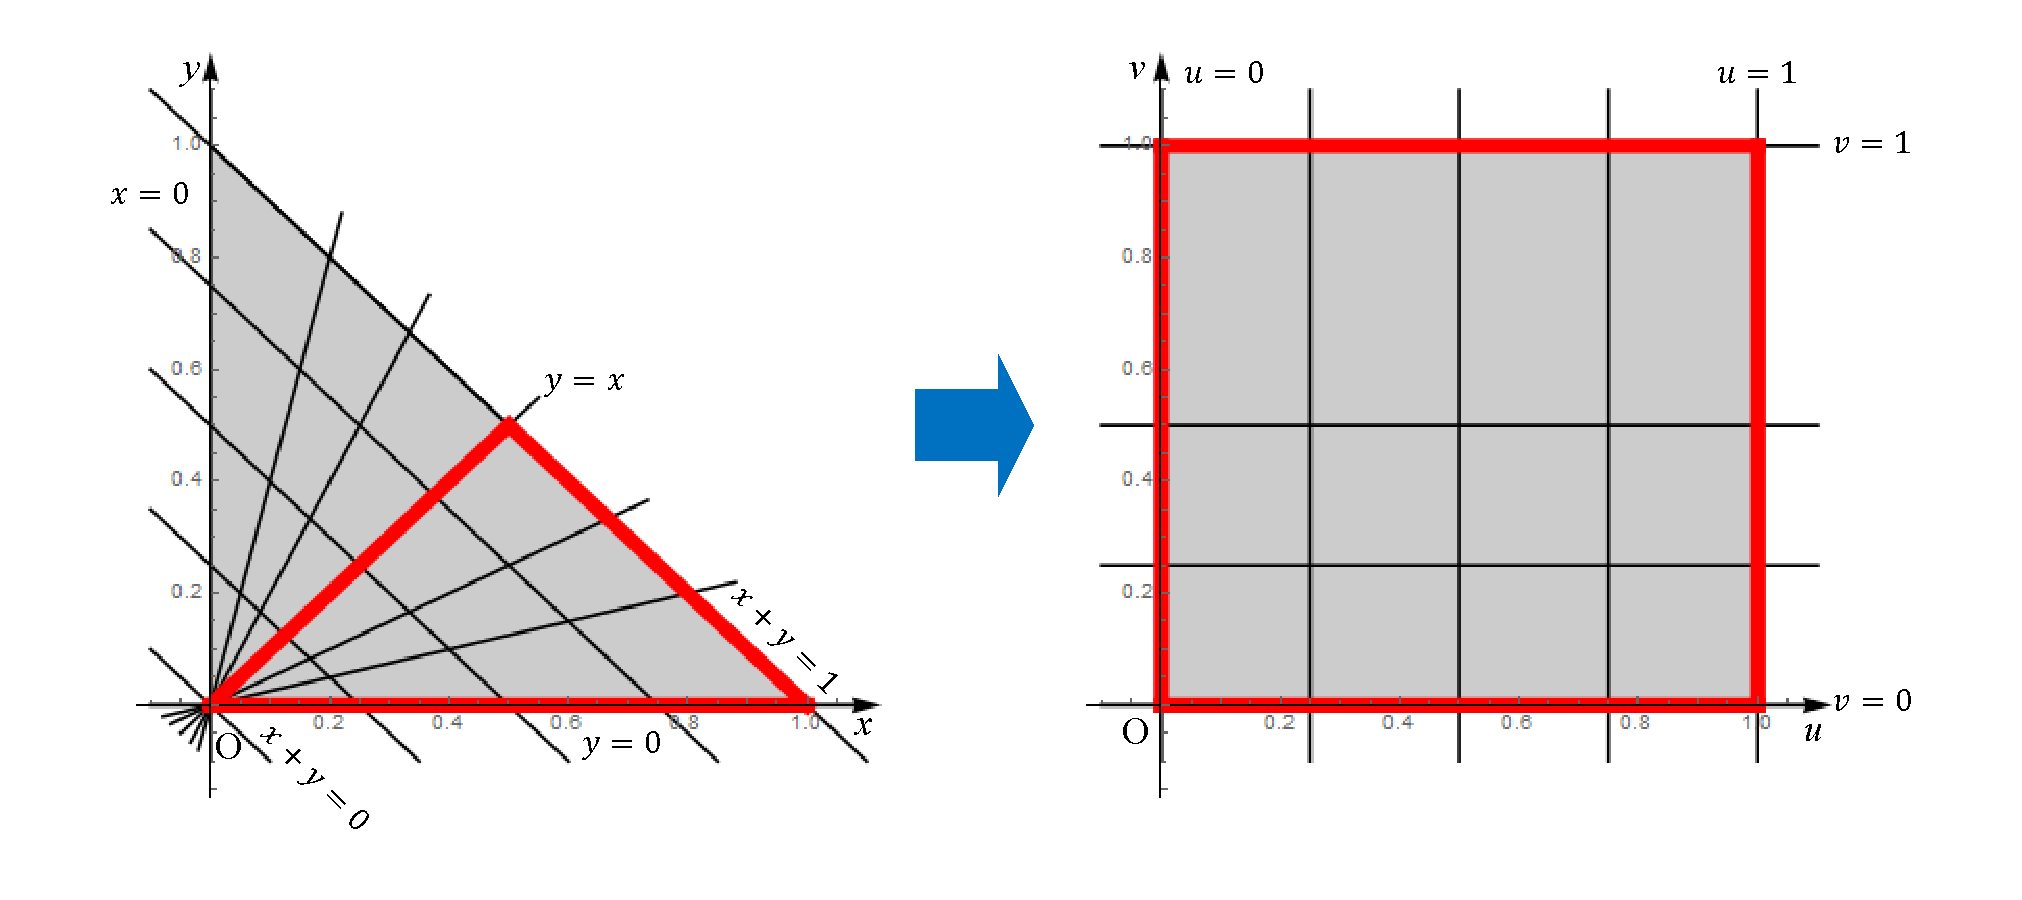
\includegraphics[height=0.3\textheight]{Figures/Fig12-3-2-1.pdf}
\end{center}
\caption{习题12.3 2题方法1图示}
\label{12-3-2-1}
\end{figure}

方法2:令$\begin{cases}
x=r\cos^2\theta,\\
y=r\sin^2\theta,
\end{cases}$则区域$D=\Set{(x,y)}{0\leqslant r\leqslant1,0\leqslant\theta\leqslant\frac\pi2}$,

$\frac{\mathrm D(x,y)}{\mathrm D(u,v)}=\begin{vmatrix}
\cos^2\theta&-2r\cos\theta\sin\theta\\
\sin^2\theta&2r\sin\theta\cos\theta
\end{vmatrix}=2r\sin\theta\cos^3\theta+2r\sin^3\theta\cos\theta=2r\sin\theta\cos\theta=r\sin2\theta$,

$\therefore I=\varIInt D{\cos(\frac{r\cos^2\theta-r\sin^2\theta}{r\cos^2\theta+r\sin^2\theta})|\frac{\mathrm D(x,y)}{\mathrm D(u,v)}|}r\theta=\varIInt D{\cos(\cos2\theta)r\sin2\theta}r\theta=\Int0{\frac\pi2}{\cos(\cos2\theta)\sin2\theta}\theta\Int01rr\\
=-\frac12\Int0{\frac\pi2}{\cos(\cos2\theta)}{\cos2\theta}\Int01rr=-\frac12\sin(\cos2\theta)\big|_0^{\frac\pi2}\frac12r^2\big|_0^1=-\frac12[\sin(-1)-\sin1]\frac12\\
=\frac12\sin1$.

{\bf注}:如图\ref{12-3-2-2}所示.\footnotemark\footnotetext{这是修订版增加的内容.}
\begin{figure}[H]
\begin{center}
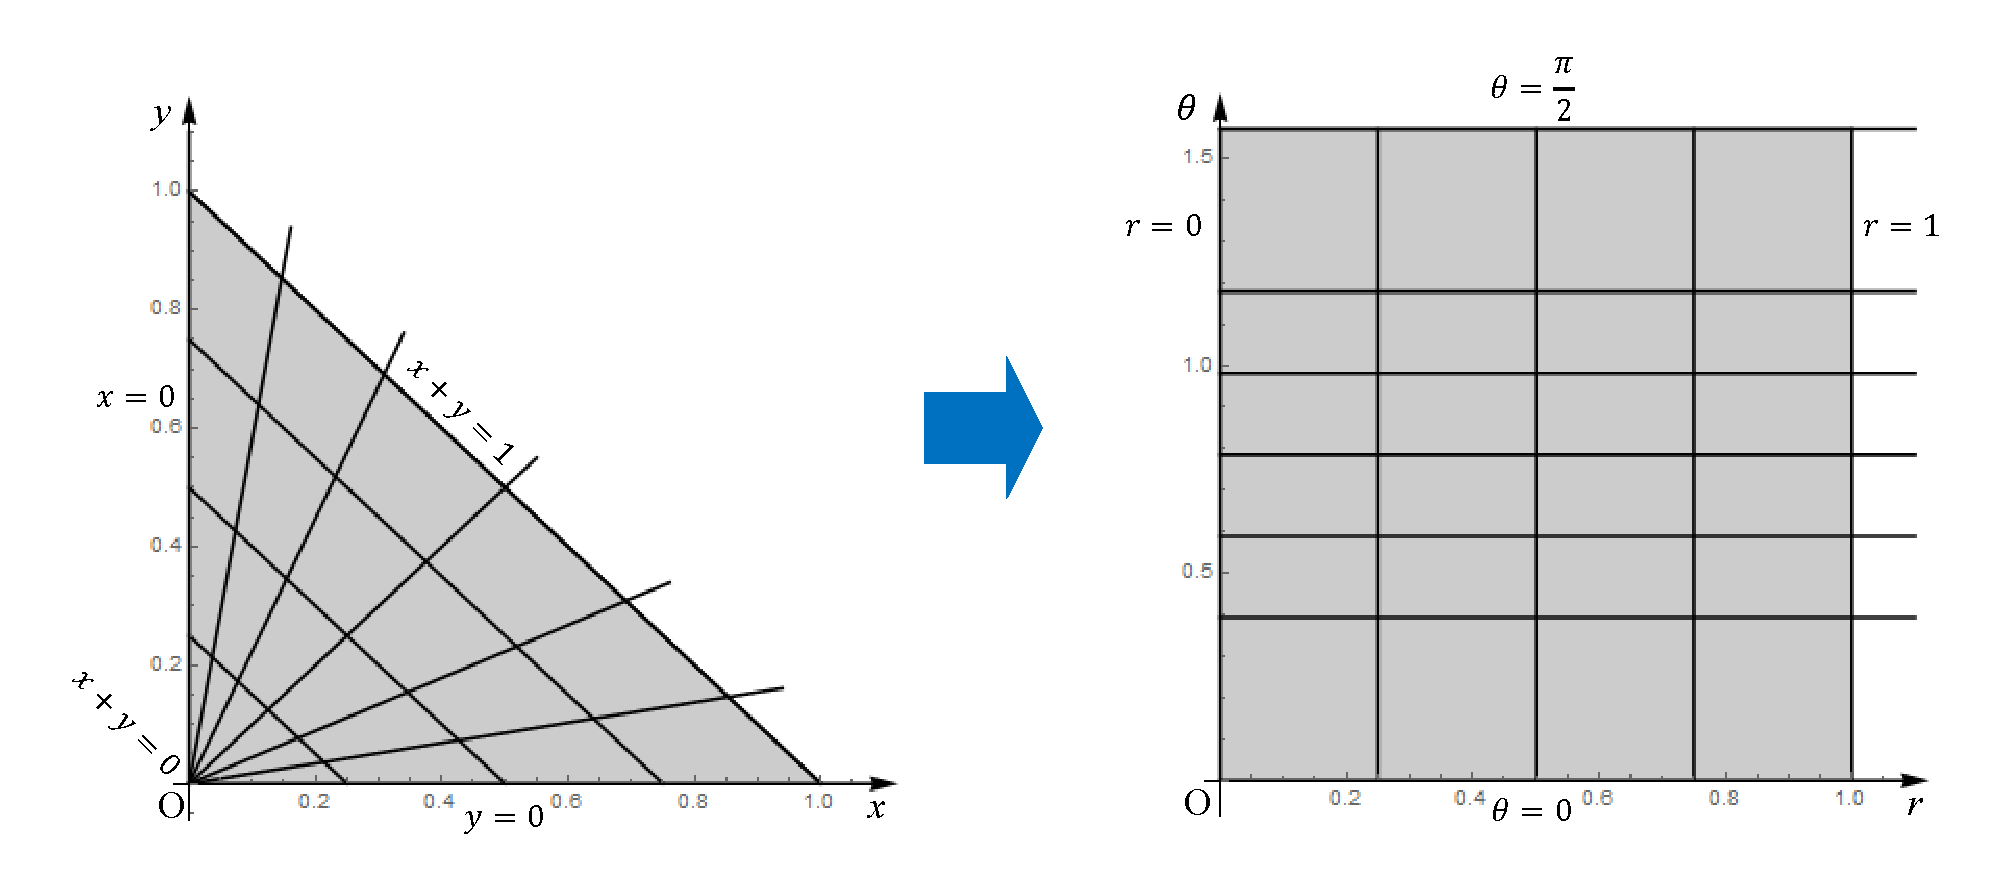
\includegraphics[height=0.3\textheight]{Figures/Fig12-3-2-2.pdf}
\end{center}
\caption{习题12.3 2题方法2图示}
\label{12-3-2-2}
\end{figure}

方法3:令$\begin{cases}
u=x-y,\\
v=x+y,
\end{cases}$则令$\begin{cases}
x=\frac12(u+v),\\
y=\frac12(v-u),
\end{cases}$区域$D=\Set{(u,v)}{0\leqslant v\leqslant1,-v\leqslant u\leqslant v}$,

$\frac{\mathrm D(x,y)}{\mathrm D(u,v)}=\begin{vmatrix}
\frac12&\frac12\\
-\frac12&\frac12
\end{vmatrix}=\frac12$,

$\therefore I=\varIInt D{\cos(\frac uv)|\frac{\mathrm D(x,y)}{\mathrm D(u,v)}|}uv=\frac12\varIInt D{\cos(\frac uv)}uv=\frac12\Int01{}v\Int{-v}v{\cos(\frac uv)}u=\frac12\Int01{}v\Int{-v}v{v\cos(\frac uv)}{\frac uv}\\
=\frac12\Int01{}v[v\sin(\frac uv)]_{-v}^v=\frac12\Int01{[v\sin1-v\sin(-1)]}v=\sin1\Int01vv=\frac12\sin1$.

注意:因为被积函数是$\cos(\frac uv)$,该函数无关于$v$初等原函数,故这种变量代换的方法应先积$u$后积$v$.

{\bf注}:如图\ref{12-3-2-3}所示.\footnotemark\footnotetext{这是修订版增加的内容.}
\begin{figure}[H]
\begin{center}
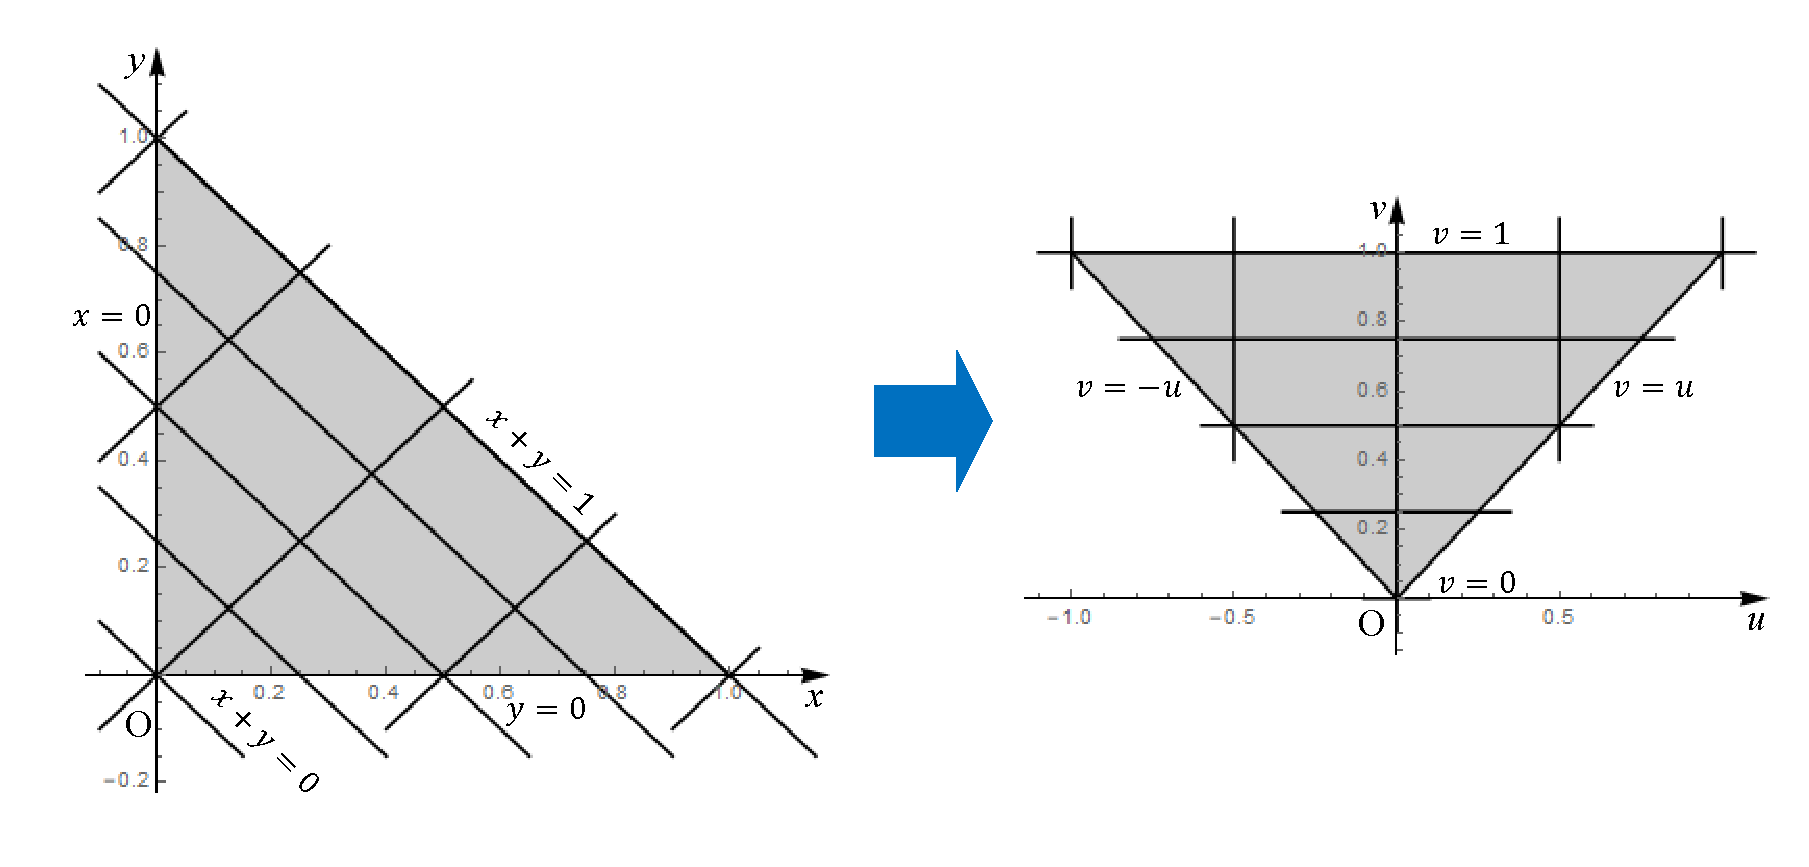
\includegraphics[height=0.3\textheight]{Figures/Fig12-3-2-3.pdf}
\end{center}
\caption{习题12.3 2题方法3图示}
\label{12-3-2-3}
\end{figure}

\item计算$I=\IInt D{(\sqrt x+\sqrt y)}\sigma,D=\Set{(x,y)}{\sqrt x+\sqrt y\leqslant1}$.

解:方法1:令$\begin{cases}
x=r^2\cos^4\theta,\\
y=r^2\sin^4\theta,
\end{cases}$则区域$D=\Set{(r,\theta)}{0\leqslant r\leqslant1,0\leqslant\theta\leqslant\frac\pi2}$,

$\frac{\mathrm D(x,y)}{\mathrm D(r,\theta)}=\begin{vmatrix}
2r\cos^4\theta&-4r^2\cos^3\theta\sin\theta\\
2r\sin^4\theta&4r^2\sin^3\theta\cos\theta
\end{vmatrix}=8r^3\sin^3\theta\cos^3\theta$,

$\therefore I=\IInt D{(\sqrt x+\sqrt y)}\sigma=\varIInt D{r|\frac{\mathrm D(x,y)}{\mathrm D(r,\theta)}|}uv=\varIInt D{8r^4\sin^3\theta\cos^3\theta}uv=\Int01{r^4}r\Int0{\frac\pi2}{2^3\sin^3\theta\cos^3\theta}\theta\\
=\frac15r^5\big|_0^1\frac12\Int0{\frac\pi2}{\sin^32\theta}{2\theta}=\frac1{10}\Int0{\frac\pi2}{\sin^32\theta}{2\theta}=\frac1{10}\Int0\pi{\sin^3\varphi}\varphi=\frac2{10}\Int0{\frac\pi2}{\sin^3\varphi}\varphi=\frac15\frac{2}{3}=\frac2{15}$.

方法2\footnotemark\footnotetext{这是修订版增加的内容.}:令$\begin{cases}
u=\sqrt x,\\
v=\sqrt y,
\end{cases}$则$\begin{cases}
x=u^2,\\
y=v^2,
\end{cases}$区域$D=\Set{(u,v)}{0\leqslant u\leqslant1,0\leqslant v\leqslant1-u}$,

$\frac{\mathrm D(x,y)}{\mathrm D(u,v)}=\begin{vmatrix}
2u&0\\
0&2v
\end{vmatrix}=4uv$,

$\therefore I=\IInt D{(\sqrt x+\sqrt y)}\sigma=\varIInt D{(u+v)|\frac{\mathrm D(x,y)}{\mathrm D(u,v)}|}uv=\varIInt D{(u+v)4uv}uv\\
=4\Int01{}u\Int0{1-u}{(u^2v+uv^2)}v=4\Int01{(\frac12u^2v^2+\frac13uv^3)\big|_0^{1-u}}u\\
=4\Int01{[\frac12u^2(1-u)^2+\frac13u(1-u)^3]}u=4\Int01{(\frac12u^2-u^3+\frac12u^4+\frac13u-u^2+u^3-\frac13u^4)}u\\
=4\Int01{(-\frac12u^2+\frac16u^4+\frac13u)}u=4(-\frac16u^3+\frac1{30}u^5+\frac16u^2)\big|_0^1=\frac2{15}$.

\item在第1象限中,设$D$由$xy=1,xy=2,\frac yx=1$及$\frac yx=4$围成,试证:
\[
\IInt D{f(xy)}\sigma=\ln2\Int12{f(x)}x.
\]
证明:令$\begin{cases}
u=xy,\\
v=\frac yx,
\end{cases}$则区域$D=\Set{(u,v)}{1\leqslant u\leqslant2,1\leqslant v\leqslant4}$,

$\frac{\mathrm D(u,v)}{\mathrm D(x,y)}=\begin{vmatrix}
y&x\\
-\frac y{x^2}&\frac1x
\end{vmatrix}=\frac yx+\frac yx=2v,\ |\frac{\mathrm D(x,y)}{\mathrm D(u,v)}|=\frac1{2v}$,

$\therefore\IInt D{f(xy)}\sigma=\varIInt D{f(u)|\frac{\mathrm D(x,y)}{\mathrm D(u,v)}|}uv=\Int12{f(u)}u\Int14{\frac1{2v}}v=\frac12\ln v\big|_1^4\Int12{f(u)}u\\
=2\ln2\Int12{f(u)}u=\ln2\Int12{f(x)}x.$
\end{enumerate}
\end{document}